\documentclass[
    letterpaper, 
    man,   
    spanish,
    12pt,
    donotrepeattitle,
    floatsintext,
    hidelinks % Opción para hyperref pasada a la clase
]{apa7}

% --- Codificación y Lenguaje ---
\usepackage[utf8]{inputenc} 
\usepackage{newunicodechar}
\usepackage[spanish]{babel} 
\selectlanguage{spanish}   
\usepackage{csquotes}       

% --- Definición de caracteres Unicode problemáticos ---
\newunicodechar{́}{'}  % U+0301 COMBINING ACUTE ACCENT
\newunicodechar{—}{---}  % U+2014 EM DASH
\newunicodechar{ć}{c'}  % U+0107 LATIN SMALL LETTER C WITH ACUTE
\newunicodechar{ı}{i}  % U+0131 LATIN SMALL LETTER DOTLESS I

% --- Bibliografía con biblatex-apa ---
\usepackage[
    style=apa,            
    backend=biber,        
    sortcites=true,       
    sorting=nyt,          
    hyperref=true,
    backref=false         
]{biblatex}
\DeclareLanguageMapping{spanish}{spanish-apa}
\addbibresource{bibliography.bib} 

% --- Paquetes para Gráficos y Tablas ---
\usepackage{graphicx}     
\usepackage{booktabs}     
\usepackage{adjustbox}    
\usepackage{multirow}     
\usepackage{array}
\usepackage{caption}
\captionsetup[figure]{labelformat=default,labelsep=period,name=Figura}
\captionsetup[table]{labelformat=default,labelsep=period,name=Tabla}
% \usepackage{epstopdf}    
% \usepackage{float}       

% --- COMANDOS PERSONALIZADOS
 \newcommand{\myparagraph}[1]{\paragraph{#1}\mbox{}\\} % Esto 
% --- Definición de comandos de tamaño de fuente ---
\renewcommand{\large}{\fontsize{14.4}{18}\selectfont}

% --- Información del Documento (Ejemplo) ---

\title{Prototipo de sistema descentralizado para la gestión y verificación de evidencias digitales en fotocomparendos aplicando Blockchain e IPFS }
\shorttitle{Gestion de Comparendos}
\author{Laura Catalina Preciado Ballen \\Cristian Stiven Guzman Tovar}
\affiliation{Universidad Distrital Francisco José de Caldas}
\course{Proyecto de grado para optar al título de: \\Ingeniero (a) de Sistemas}
\professor{Julio Baron Velandia}
\duedate{\today}
\abstract{Este trabajo propone el diseño e implementación de un prototipo basado en Blockchain para la gestión de fotocomparendos en Bogotá, con el objetivo de garantizar la transparencia del proceso. Se utilizarán contratos inteligentes para registrar cada infracción, permitiendo que cualquier actor autorizado pueda verificar su autenticidad sin necesidad de intermediarios. Mediante pruebas y simulaciones, se evaluará la viabilidad del sistema, demostrando cómo esta tecnología puede fortalecer la confianza en los procesos de control de tránsito y mejorar la eficiencia en la gestión de sanciones. }
\keywords{Fotocomparendos, Gestion de datos, Blockchain, ingeniería web}

\begin{document}
% \maketitle
%Preguntar cual dejar?
\begin{titlepage}
    \begin{center}
        \vspace*{0.5cm}
            
        \Large
        \textbf{Prototipo de sistema descentralizado para la gestión y verificación de evidencias digitales en fotocomparendos aplicando Blockchain e IPFS}
            
        
        \vspace{2.5cm}
            
        \normalsize
        \textbf{Laura Catalina Preciado Ballen}\\
        \textbf{Cristian Stiven Guzman Tovar}
            
        \vfill
            
        Proyecto de Monografía para Optar por el Título de\\
        Ingeniero(a) de Sistemas
            
        \vspace{0.8cm}
            
        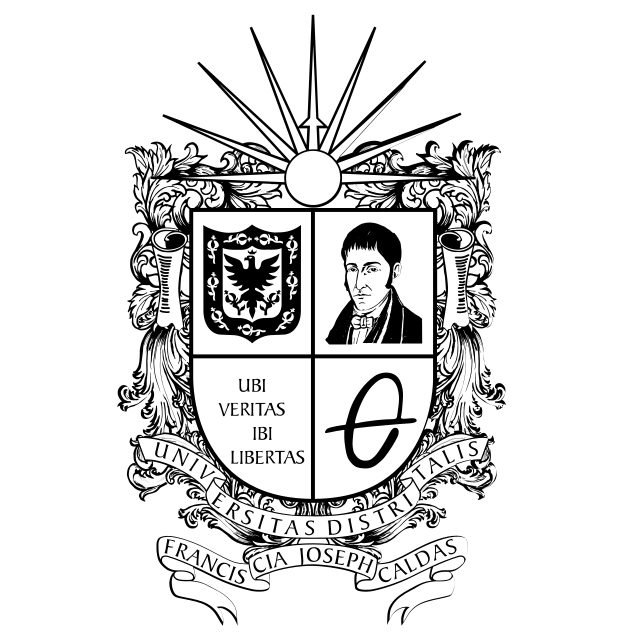
\includegraphics[width=0.2\textwidth]{Images/Escudo_UD}
            
        \large
        Universidad Distrital Francisco José De Caldas\\
        Facultad de Ingeniería\\
        Colombia, Bogotá D.C.\\
        Julio de 2025\\

        
            
    \end{center}
\end{titlepage}

\raggedbottom 

\pagenumbering{roman}
    % Contenido
\renewcommand\contentsname{\textbf{Índice}}
\tableofcontents
\setcounter{tocdepth}{2}
\newpage
    % Fíguras
\renewcommand{\listfigurename}{\textbf{Índice de figuras}}
\listoffigures
\newpage
    % Tablas
\renewcommand{\listtablename}{\textbf{Índice de tablas}}
\listoftables
\newpage

% Cuerpo
\pagenumbering{arabic}

% Incluir capítulos modularizados
\section{\large Introducción}
En Colombia, la gestión de fotocomparendos ha sido objeto de controversia debido a fallas en la transparencia y posibles manipulaciones en el proceso de registro y validación de infracciones. La falta de un sistema confiable ha generado desconfianza entre los ciudadanos, lo que evidencia la necesidad de una solución que garantice la integridad, inmutabilidad y verificabilidad de la información.

La tecnología Blockchain ha demostrado ser una alternativa eficaz para el almacenamiento seguro y descentralizado de datos, asegurando que una vez registrados, estos no puedan ser alterados sin dejar rastro. A través de contratos inteligentes, es posible automatizar la validación y el procesamiento de fotocomparendos, reduciendo la intervención humana y minimizando el riesgo de corrupción o errores administrativos.

Este trabajo propone el diseño e implementación de un prototipo basado en Blockchain para la gestión de fotocomparendos en Bogotá, con el objetivo de garantizar la transparencia del proceso. Se utilizarán contratos inteligentes para registrar cada infracción, permitiendo que cualquier actor autorizado pueda verificar su autenticidad sin necesidad de intermediarios. Mediante pruebas y simulaciones, se evaluará la viabilidad del sistema, demostrando cómo esta tecnología puede fortalecer la confianza en los procesos de control de tránsito y mejorar la eficiencia en la gestión de sanciones.

\subsection{Formulación del problema}
El sistema actual de gestión de fotocomparendos en Bogotá, enfrenta serias limitaciones en términos de transparencia, seguridad e integridad de la información, lo que genera desconfianza por parte de la ciudadanía y dificultades administrativas en su gestión. Según el Observatorio de Movilidad de Bogotá, entre enero de 2018 y agosto de 2024 se emitieron 5.575.982 comparendos, de los cuales el 48,91 \% fueron generados mediante dispositivos electrónicos de asistencia policial \parencite{ObservatorioComparendos2025}

\begin{figure}[htbp]
    \begin{flushleft}
        \textbf{Figura 1}\\
        \textit{Estadísticas de comparendos emitidos en Bogotá entre enero de 2018 y agosto de 2024}
    \end{flushleft}
    \centering
    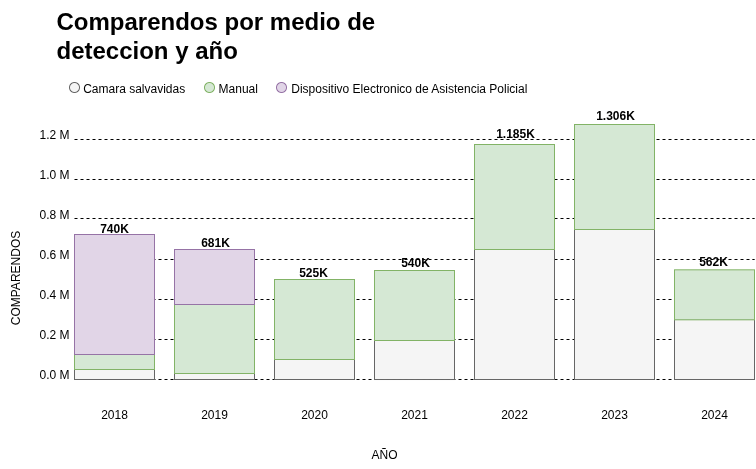
\includegraphics[width=0.8\textwidth]{Images/numComparendos.png}
    \vspace{0.5em}
    \begin{flushleft}
        \textit{Nota.} Tomado del Observatorio de Movilidad de Bogotá.
    \end{flushleft}
    \label{fig:estadisticas_comparendos}
\end{figure}

Estas cifras reflejan el papel protagónico que tienen las fotomultas en la regulación del tránsito en la ciudad, pero también resaltan la necesidad urgente de fortalecer los mecanismos de manejo, almacenamiento y verificación de evidencias.  

La ausencia de un sistema confiable y auditable que permita garantizar la inmutabilidad de los registros, así como la trazabilidad de las evidencias, ha generado un entorno donde se cuestiona la validez de las sanciones, se incrementan las quejas ciudadanas y se limita la eficiencia operativa de las entidades encargadas del control de tránsito. En este contexto, surge la necesidad de explorar tecnologías emergentes, como Blockchain e IPFS, que podrían ofrecer una solución más segura, descentralizada y transparente para la gestión de estos procesos. 

\subsection{Objetivos}
\paragraph{Objetivo General}
Desarrollar un prototipo que gestione los foto comparendos en Bogota, utilizando tecnologías como Hyperledger Fabric e InterPlanetary File System con el fin de tener una gestión segura, auditable y descentralizada del  proceso. 

\paragraph{Objetivos específicos}
\begin{itemize}
    \item Analizar el proceso actual de gestión de fotocomparendos en Bogotá, mediante la revisión de la normativa y una auditoria del sistema Fenix -El istema que actualmnte gestiona los fotocomparendos en Bogota- para identificar las vulnerabilidades y los requisitos funcionales y no funcionales (seguridad, rendimiento y auditabilidad) que el prototipo debe satisfacer, resultando en una lista de requerimientos específicos para la nueva solución.
    \item Construir el prototipo del sistema de gestión de foto comparendos, implementando la arquitectura propuesta (InterPlanetary File System para almacenamiento de imágenes y Hyperledger Fabric para el registro de transacciones), asegurando que cada transacción contenga el hash único de InterPlanetary File System y los metadatos esenciales del comparendo (fecha, hora, lugar, placa, tipo de infracción), y desarrollando una interfaz básica que permita la carga de la evidencia y la consulta/verificación de los registros en la blockchain y la imagen en InterPlanetary File System, con el fin de materializar técnicamente la solución propuesta basada en los requisitos identificados en el objetivo anterior.
    \item Evaluar la efectividad y viabilidad del prototipo desarrollado, mediante la ejecución de un plan de pruebas funcionales (verificar la correcta carga a InterPlanetary File System, el registro inmutable en el ledger, la consistencia de datos, la capacidad de verificación) y pruebas de rendimiento básicas (medir tiempos de registro y consulta) en un entorno de simulación controlado, para validar que el prototipo cumple con los requisitos clave de inmutabilidad, transparencia y seguridad.
\end{itemize} 
\section{\large Justificación}
La gestión actual de los fotocomparendos en Bogotá, centralizada en el sistema Fénix, presenta graves limitaciones de seguridad y transparencia que han erosionado la confianza pública en el proceso sancionatorio. Esta se manifiesta en un riesgo sistémico de corrupción, un fenómeno documentado tanto a nivel internacional, como el escándalo de «ticket-fixing» en Nueva York, como a nivel nacional, donde existen redes ilícitas que manipulan y eliminan comparendos en el sistema \parencite{barbaro2011ticketfixing, blogAletta, procuraduriaBucaramanga}.

La raíz de este problema reside en la arquitectura centralizada de las bases de datos tradicionales, que permite a personal interno modificar registros sin dejar un rastro auditable, comprometiendo la integridad de todo el proceso. Esta debilidad se ve agravada por las deficiencias en ciberseguridad identificadas en el \textit{Informe Final de Auditoría AC-SDM-090 de 2023}, que señala controles de acceso insuficientes y falta de monitoreo en los sistemas de la Secretaría de Movilidad \parencite{auditoriaSDM}. Estas falencias no solo incrementan el riesgo de ataques, sino que debilitan la capacidad institucional para defender la legitimidad de las sanciones impuestas.
Estas diferencias estructurales entre el modelo centralizado actual y la alternativa descentralizada se resumen en la Tabla~\ref{tab:comparacion_bd_blockchain}, evidenciando las ventajas de Blockchain en términos de seguridad, integridad y gobernanza de datos:

\begin{table}[htbp]
    \begin{flushleft}
        \textbf{Tabla 1}\\[2em]
        \textit{Comparación entre bases de datos tradicionales y blockchain para gestión de registros gubernamentales}
    \end{flushleft}
    \vspace{1em}
    \addcontentsline{lot}{table}{Tabla 1. Comparación entre bases de datos tradicionales y blockchain para gestión de registros gubernamentales}
    \centering
    \begin{tabular}{p{4.5cm} p{5.2cm} p{5.2cm}}
        \toprule
        \textbf{Característica} & \textbf{Base de Datos Convencional} & \textbf{Blockchain} \\
        \midrule
        Modelo de confianza & Se basa en un administrador central (entidad de TI) & Confianza distribuida entre múltiples nodos \\
        Inmutabilidad & Registros pueden ser modificados o eliminados por administradores & Los registros son inmutables por diseño \\
        Trazabilidad / Auditoría & Depende de la implementación y control interno & Historial completo e inalterable disponible \\
        Riesgo de corrupción interna & Alto, si hay privilegios indebidos o colusión & Bajo, no se puede alterar sin consenso de la red \\
        Seguridad criptográfica & Opcional, no siempre integrada nativamente & Integrada (firmas digitales, hashes, cifrado) \\
        Disponibilidad / tolerancia a fallos & Riesgo de puntos únicos de falla & Alta disponibilidad por replicación descentralizada \\
        Velocidad de operación & Alta velocidad en lectura/escritura & Menor velocidad, prioriza integridad y consenso \\
        \bottomrule
    \end{tabular}
    \vspace{2em}
    \begin{flushleft}
        \textit{Nota.} Elaboración propia.
    \end{flushleft}
    \refstepcounter{table}\label{tab:comparacion_bd_blockchain}
\end{table}

Frente a este escenario, la tecnología Blockchain, en conjunto con IPFS, ofrece un cambio de paradigma hacia un modelo más seguro y transparente. Como se observa en la comparación, a diferencia de un sistema centralizado donde la confianza recae en una única entidad falible, una solución Blockchain distribuye los datos en una red criptográficamente enlazada. Esto garantiza que cada registro, una vez validado, sea inmutable y verificable por todas las partes autorizadas, haciendo que cualquier intento de alteración sea computacionalmente inviable y fácilmente detectable. Se elimina así la dependencia de intermediarios y se crea una fuente única y confiable de verdad.

En síntesis, la adopción de este prototipo se justifica por su capacidad para:
\begin{itemize}
\item \textbf{Mitigar la corrupción}, al garantizar la integridad de los datos y eliminar la posibilidad de manipulación unilateral.
\item \textbf{Fortalecer la seguridad de la información}, mediante una arquitectura distribuida y tolerante a fallos.
\item \textbf{Aumentar la confianza ciudadana}, al ofrecer mecanismos transparentes y auditables para la validación de infracciones.
\item \textbf{Optimizar los procesos administrativos}, automatizando registros, auditorías y la verificación de evidencias.
\end{itemize}

Esta propuesta no solo responde a desafíos técnicos y éticos urgentes en Bogotá, sino que también se alinea con las tendencias globales en gobernanza digital (\textit{GovTech}), sentando un precedente innovador para la gestión de sanciones públicas con mayor fiabilidad y transparencia.
\section{\large Marco Teórico}
El marco conceptual y tecnologico que sustenta la propuesta del prototipo, presentan las teorías y modelos clave que justifican la selección de Blockchain e IPFS como componentes centrales, evidencian los principios inherentes de integridad, transparencia, resiliencia y auditabilidad en la gestión de evidencia digital crítica como los fotocomparendos.
\subsection{El Paradigma de la Confianza Descentralizada}
Los sistemas de información tradicionales suelen depender de intermediarios centralizados o autoridades certificadoras para validar transacciones y garantizar la fiabilidad de los registros. La teoría de los modelos de confianza descentralizada, en cambio, analiza cómo establecer y mantener la confianza en entornos distribuidos donde tales autoridades centrales están ausentes \parencite{swan2015blockchain}.

La relevancia de este modelo es fundamental para justificar el uso de la tecnología Blockchain en la gestión de fotocomparendos, ya que su propósito es precisamente reemplazar la necesidad de depositar confianza exclusiva en una única entidad para la custodia, validación e integridad de los registros. Blockchain habilita un cambio de paradigma: en lugar de confiar en un actor central, la confianza se distribuye y se deposita en la robustez del protocolo criptográfico subyacente \parencite{nakamoto2008bitcoin}, en la transparencia de las reglas del sistema y en el consenso mayoritario de los participantes de la red \parencite{antonopoulos2023mastering}. Este enfoque reduce drásticamente los puntos únicos de fallo y los vectores de corrupción asociados a la dependencia de intermediarios centralizados, quienes podrían ser comprometidos, cometer errores o actuar de manera malintencionada.

\subsection{Fundamentos de los Sistemas Distribuidos y Redes Descentralizadas}
El paradigma de la confianza descentralizada se sustenta en la teoría de los sistemas distribuidos, donde múltiples entidades autónomas, denominadas nodos, colaboran a través de una red para alcanzar un objetivo común, compartiendo tanto la carga computacional como el almacenamiento de datos \parencite{vanSteen2017}. Estos sistemas se fundamentan en principios como la distribución de recursos, la comunicación inter-nodo y mecanismos de coordinación que prescinden de intermediarios centrales \parencite{coulouris2011}.

La relevancia de esta teoría para el presente proyecto es primordial, ya que tanto Blockchain como el InterPlanetary File System (IPFS) son implementaciones nativas de sistemas distribuidos. Su adopción conjunta promueve inherentemente:
\begin{itemize}
    \item \textbf{Resiliencia:} Al eliminar puntos únicos de fallo (Single Points of Failure - SPOF).
    \item \textbf{Alta Disponibilidad:} Al permitir el acceso a datos y servicios desde múltiples nodos.
    \item \textbf{Resistencia a la Censura:} Dado que ninguna entidad individual posee control absoluto sobre la red o los datos almacenados \parencite{antonopoulos2023mastering}.
\end{itemize}

Una característica esencial de estos sistemas es su arquitectura de red \textbf{Peer-to-Peer (P2P)}, donde los participantes se conectan y comparten recursos directamente entre sí, sin necesidad de un servidor central. En una red P2P, cada nodo puede actuar simultáneamente como cliente y servidor, lo que posibilita que el registro distribuido (ledger) se mantenga sincronizado y que los archivos puedan ser recuperados desde múltiples fuentes, garantizando la integridad de la información sin depender de una autoridad central.

\subsection{Tecnologías para la Gestión Descentralizada de Evidencia}
Para materializar un sistema de gestión de fotocomparendos descentralizado, se requiere la sinergia de dos tipos de tecnologías: una para el registro inmutable de transacciones y otra para el almacenamiento verificable de la evidencia.

\subsubsection{Blockchain: Un Registro Distribuido, Inmutable y Transparente}
Blockchain es un tipo específico de Tecnología de Ledger Distribuido (DLT), un sistema de registro digital caracterizado por ser distribuido, sincronizado y asegurado criptográficamente entre múltiples participantes \parencite{narayanan2016bitcoin}. Su estructura fundamental se compone de \textbf{transacciones} —operaciones firmadas digitalmente que modifican el estado del ledger de forma permanente \parencite{antonopoulos2023mastering}— agrupadas en bloques. Cada bloque contiene un hash criptográfico que lo vincula al anterior, formando una cadena cronológica e inmutable.

La \textbf{inmutabilidad} y la \textbf{transparencia} son los beneficios centrales que esta tecnología aporta \parencite{swan2015blockchain,antonopoulos2023mastering}. La primera se logra mediante la estructura encadenada y los mecanismos de consenso distribuido (ej., Proof-of-Work \parencite{nakamoto2008bitcoin} o Proof-of-Stake \parencite{king2012ppcoin}), que hacen que la modificación de un bloque pasado sea computacionalmente prohibitiva. La segunda se habilita por la naturaleza replicada del ledger, permitiendo que actores autorizados puedan consultar y verificar la información de forma independiente. Dentro de este ecosistema, los \textbf{Smart Contracts} (Contratos Inteligentes) actúan como programas autoejecutables cuyo código define e impone automáticamente los términos de un proceso, permitiendo automatizar la gestión del ciclo de vida del comparendo \parencite{szabo1997smart, wood2014ethereum, buterin2014next}.

\paragraph{Modelos Arquitectónicos y Elección para el Prototipo.}
La tecnología Blockchain no es monolítica; existen diferentes arquitecturas:
\begin{itemize}
    \item \textbf{Públicas (Permissionless):} Abiertas a cualquier participante, priorizan la descentralización radical (ej. Bitcoin, Ethereum) \parencite{nakamoto2008bitcoin}.
    \item \textbf{Privadas:} Controladas por una única entidad, ofrecen alta eficiencia pero son centralizadas.
    \item \textbf{De Consorcio/Permisionadas (Permissioned):} Operadas por un grupo selecto de participantes autorizados. Ofrecen un equilibrio entre descentralización, rendimiento y confidencialidad, siendo la opción ideal para contextos gubernamentales y empresariales \parencite{vukolic2015quest,cachin2018architecture}.
\end{itemize}
Para este prototipo, se opta por una \textbf{implementación permisionada} (simulada con Hyperledger Fabric), permitiendo que solo entidades autorizadas operen nodos y registren transacciones, con un mecanismo de consenso eficiente (ej. Raft) adecuado para un sistema de gestión de registros.

\subsubsection{IPFS: Almacenamiento Verificable mediante Direccionamiento por Contenido}
Los ledgers de Blockchain no están optimizados para almacenar grandes volúmenes de datos (blobs), como las imágenes de los fotocomparendos \parencite{xu2019taxonomy}. Para resolver esto, se utiliza un sistema de almacenamiento descentralizado. La elección de IPFS sobre alternativas centralizadas como AWS S3 es crucial para la integridad del sistema. Mientras que en un sistema centralizado el propietario puede modificar o eliminar unilateralmente un archivo \parencite{vogels2008eventually}, IPFS opera bajo el paradigma del \textbf{direccionamiento por contenido (Content Addressing)} \parencite{benet2014ipfs, voigt2017gdpr}.

En este modelo, la identidad única de un archivo, su Content Identifier (CID), es un \textbf{hash criptográfico} derivado directamente de su contenido. Esto establece un vínculo intrínseco e inmutable: si el contenido del archivo cambia, incluso mínimamente, su CID también cambiará. IPFS es un protocolo y red P2P que utiliza este principio: divide los archivos en bloques, calcula sus hashes y permite su recuperación a través de su CID, utilizando mecanismos como DHT para localizar los nodos que los poseen \parencite{maymounkov2002kademlia, benet2014ipfs}.

\subsection{Arquitectura de la Solución: Sinergia Blockchain-IPFS con el Transacción Off-Chain}
La integración de ambas tecnologías se materializa mediante el patrón de almacenamiento \textbf{off-chain}. El flujo de trabajo es el siguiente:
\begin{enumerate}
    \item La imagen probatoria del comparendo se carga a un nodo IPFS, obteniendo su CID único.
    \item Se crea una transacción en la Blockchain (on-chain) que contiene este CID junto con los metadatos esenciales del comparendo (fecha, hora, lugar, placa).
    \item Esta transacción se valida y registra de forma inmutable en el ledger.
\end{enumerate}
Este enfoque crea un enlace criptográfico inalterable entre el registro oficial (en Blockchain) y la evidencia visual original (en IPFS). Cualquier intento de manipulación de la imagen almacenada en IPFS resultaría en un CID diferente, rompiendo explícitamente la cadena de custodia digital y haciendo que la alteración sea detectable de forma inmediata y algorítmica. La combinación de Blockchain e IPFS no solo sigue los principios de descentralización \parencite{vanSteen2017}, sino que refuerza activamente los objetivos de inmutabilidad verificable y transparencia del sistema.

\subsection{Fundamentos Criptográficos Aplicados}
La criptografía proporciona los pilares matemáticos que garantizan la seguridad, integridad y autenticidad en todo el ecosistema del prototipo \parencite{katz2020introduction}.
\begin{itemize}
    \item \textbf{Funciones Hash Criptográficas:} Son algoritmos que transforman datos en una huella digital de tamaño fijo. Sus propiedades (unidireccionalidad, resistencia a colisiones, efecto avalancha) son vitales \parencite{schneier2007applied, menezes1996handbook}. En este proyecto, se utilizan para: generar el CID en IPFS, asegurar la integridad de la cadena de bloques y crear identificadores únicos para las transacciones \parencite{benet2014ipfs, nakamoto2008bitcoin}.
    \item \textbf{Criptografía Asimétrica y Firmas Digitales:} Basada en pares de claves (pública y privada), habilita las firmas digitales \parencite{diffie2022new, rivest1978method}. Cuando un usuario autorizado registra un comparendo, utiliza su clave privada para firmar la transacción. Cualquier participante puede usar la clave pública correspondiente para verificar la firma, garantizando así la \textbf{autenticidad} y el \textbf{no repudio} de la acción \parencite{katz2020introduction}.
\end{itemize}
\section{\large Marco Conceptual}
Este marco conceptual define los elementos tecnológicos, componentes y términos clave que constituyen el "Prototipo para la Gestión de Fotocomparendos mediante Tecnología Blockchain". Su objetivo es proporcionar una comprensión clara y precisa del "qué" de cada componente utilizado en el sistema propuesto. 

\paragraph{Blockchain / Tecnología de Ledger Distribuido (DLT)}
Una blockchain es un tipo específico de Tecnología de Ledger Distribuido (Distributed Ledger Technology, DLT), un sistema de registro digital caracterizado por ser distribuido, sincronizado y asegurado criptográficamente entre múltiples participantes \parencite{narayanan2016bitcoin}. La estructura fundamental se compone de bloques de datos que contienen transacciones validadas y un hash criptográfico que lo vincula al bloque anterior, formando una cadena cronológica. La red está mantenida por nodos que almacenan copias del ledger y ejecutan un protocolo de consenso (ej., Proof-of-Work descrito por \parencite{nakamoto2008bitcoin}, o Proof-of-Stake por \parencite{king2012ppcoin}) para validar y agregar nuevos bloques. Las características clave resultantes son la descentralización, la inmutabilidad (resistencia a la alteración de datos pasados), la transparencia configurable y la seguridad criptográfica \parencite{swan2015blockchain}. DLT es el término general, mientras que Blockchain se refiere específicamente a la estructura de bloques encadenados \parencite{ukgov2016dlt}.

\paragraph{Transacción (en Blockchain)} 

En el contexto de Blockchain, una transacción es una operación firmada digitalmente que se propaga a la red para su validación e inclusión en un bloque \parencite{antonopoulos2023mastering}. Una vez confirmada, modifica el estado del ledger de forma permanente. Para este proyecto, cada transacción crucial encapsula el hash CID de la imagen del comparendo obtenida de IPFS y los metadatos asociados (ej., fecha, lugar, placa, infracción). Funciona como el registro inmutable que vincula la prueba visual con los datos descriptivos del evento. 

\paragraph{Redes P2P (Peer-to-Peer)} 

 Una red P2P (del inglés Peer-to-Peer, o red entre pares) es un modelo de arquitectura de red en el que los participantes, denominados "pares" o "nodos", se conectan y comparten recursos directamente entre sí, sin necesidad de un servidor central que actúe como intermediario. A diferencia del modelo cliente-servidor tradicional, en una red P2P cada nodo puede actuar simultáneamente como cliente y como servidor. 

En el contexto de este proyecto, el paradigma P2P es fundamental, ya que es la base sobre la que se construyen tanto la tecnología Blockchain como el sistema IPFS. Este modelo permite la descentralización inherente al sistema, eliminando los puntos únicos de fallo y aumentando la resiliencia y la resistencia a la censura. La comunicación directa entre nodos es lo que posibilita que el ledger se mantenga sincronizado y que los archivos en IPFS puedan ser recuperados desde múltiples fuentes, garantizando la disponibilidad y la integridad de la información sin depender de una autoridad central. 
\paragraph{IPFS (InterPlanetary File System)} 

IPFS es un protocolo y red P2P diseñado para el almacenamiento y la compartición de archivos distribuida y direccionable por contenido \parencite{benet2014ipfs}. Su funcionamiento básico implica dividir archivos en bloques, calcular el hash de cada bloque y construir una estructura de datos Merkle DAG cuyo hash raíz es el CID del archivo. Para almacenar, un nodo anuncia los hashes de los bloques que posee. Para recuperar, un nodo solicita el archivo por su CID, y la red IPFS utiliza mecanismos como DHT \parencite{maymounkov2002kademlia} para localizar y obtener los bloques de los nodos pares que los poseen \parencite{benet2014ipfs}. 

\paragraph{Hash Criptográfico (y Hash Único/CID)} 

Un hash criptográfico es una salida de longitud fija generada por una función hash a partir de una entrada de datos, actuando como su huella digital única \parencite{menezes1996handbook}. Debe ser resistente a colisiones y unidireccional. Su aplicación en el proyecto es doble: En IPFS, como Content Identifier (CID), identifica unívocamente la imagen del comparendo, asegura su integridad y permite su recuperación \parencite{benet2014ipfs}. En Blockchain, se utiliza para enlazar bloques (asegurando la integridad de la cadena) y para identificar transacciones \parencite{nakamoto2008bitcoin}. 

\paragraph{Metadatos}  

Los metadatos son «datos acerca de datos» \parencite{gilliland2008setting}. En este proyecto, se refieren a la información estructurada que describe el contexto del fotocomparendo (fecha, hora, lugar, tipo de infracción, placa, etc.). Estos metadatos se registran directamente en la transacción Blockchain, junto al CID de la imagen, proporcionando un contexto inmutable y fácilmente verificable para la evidencia visual. 

\paragraph{Smart Contract (Contrato Inteligente)} 

Un Smart Contract es un programa autoejecutable almacenado en una Blockchain, cuyo código define e impone automáticamente los términos de un acuerdo o proceso cuando se cumplen condiciones predefinidas \parencite{szabo1997smart, wood2014ethereum}. Su aplicación potencial en este proyecto podría extenderse a la gestión automatizada del ciclo de vida del comparendo (actualización de estado de pago, aplicación de plazos o sanciones) o a la implementación de reglas de acceso y auditoría más complejas \parencite{buterin2014next}. 

\paragraph{Proceso de Verificación Digital (en este contexto)}  

Este proceso se refiere a los pasos técnicos para confirmar la autenticidad e integridad de un fotocomparendo usando las tecnologías del prototipo. El mecanismo implica: consultar la transacción en la Blockchain mediante un identificador, extraer el CID y los metadatos registrados, usar el CID para recuperar la imagen original de IPFS, y permitir al usuario comparar la información. La fiabilidad del proceso se basa en la inmutabilidad de la Blockchain \parencite{nakamoto2008bitcoin} y el direccionamiento por contenido de IPFS \parencite{benet2014ipfs}, que conjuntamente aseguran que tanto el registro como la evidencia visual son auténticos y no han sido alterados. 
\section{\large Estado del Arte}  

\subsection{Blockchain para Registros Gubernamentales y Gestión de Sanciones} 

La aplicación de la tecnología Blockchain y DLT (Distributed Ledger Technology) en la administración pública ha sido un área de creciente interés, impulsada por las promesas teóricas de Inmutabilidad, Transparencia y Auditoría mejorada, fundamentales para la Confianza Descentralizada. La investigación sugiere que Blockchain puede transformar la gestión de registros oficiales, como licencias, títulos de propiedad y, potencialmente, multas o sanciones como los fotocomparendos. 

\paragraph{Análisis de Aplicación}
La capacidad de crear un registro de Transacciones criptográficamente asegurado y distribuido permite generar una pista de auditoría fiable y resistente a la manipulación. Cada registro de sanción, incluyendo sus Metadatos (fecha, hora, ubicación, tipo de infracción) y el Hash de la evidencia asociada, puede ser anclado a la cadena, proporcionando una fuente única de verdad verificable por las partes autorizadas. Esto se alinea con los principios de Sistemas Distribuidos aplicados a la gobernanza. 

\paragraph{Blockchains Públicas vs. Permisionadas}
En el contexto gubernamental, la literatura y los estudios piloto tienden a favorecer las blockchains permisionadas (o de consorcio). Si bien las blockchains públicas ofrecen máxima transparencia, las permisionadas permiten a las entidades gubernamentales controlar quién puede participar en la red (validar transacciones, acceder a datos), gestionar mejor la privacidad (crucial para datos ciudadanos) y, a menudo, ofrecer mayor rendimiento y escalabilidad. La elección impacta directamente en el modelo de Confianza Descentralizada implementado. 

\paragraph{Madurez y Barreras}
Aunque existen numerosos estudios y proyectos piloto (ej., registros de tierras en Suecia o Georgia, identidad digital en Estonia), las implementaciones a gran escala para la gestión integral de sanciones administrativas aún son limitadas. La madurez es variable. Las barreras reconocidas incluyen la complejidad técnica, la necesidad de marcos legales y regulatorios adaptados, la interoperabilidad con sistemas heredados, los costos iniciales de implementación y la adopción tanto por parte de las instituciones como de los ciudadanos. La Percepción Pública de la Tecnología Blockchain también juega un rol significativo. 

\subsection{Integración de Blockchain e IPFS para Datos Voluminosos y Verificables} 

El almacenamiento directo de datos voluminosos (como imágenes o vídeos de alta resolución) en una Blockchain es ineficiente y costoso. La literatura técnica y diversos prototipos exploran la integración de Blockchain con sistemas de Almacenamiento Direccionable por Contenido como IPFS (InterPlanetary File System) para abordar este desafío. 

\paragraph{Estado Actual} El enfoque predominante consiste en almacenar el dato voluminoso (la imagen del fotocomparendo) en IPFS, obteniendo un Hash único basado en su contenido. Este Hash IPFS, junto con otros Metadatos relevantes, se almacena en una Transacción Blockchain. Este modelo aprovecha la eficiencia de IPFS para el almacenamiento distribuido y la fortaleza de Blockchain para el registro inmutable y verificable del puntero (el Hash) y los metadatos asociados. 

\paragraph{Ventajas y Desafíos} Las ventajas logradas incluyen la verificabilidad (cualquier cambio en el archivo IPFS cambiaría su hash, invalidando el enlace en la Blockchain), la resiliencia potencial (si múltiples nodos almacenan el archivo) y el direccionamiento por contenido inherente a IPFS. Sin embargo, persisten desafíos persistentes significativos: 

\paragraph{Persistencia de Datos (Pinning)} Los datos en IPFS solo persisten mientras algún nodo los esté "pineando" (almacenando activamente). Garantizar la persistencia a largo plazo de la evidencia requiere mecanismos o servicios de pinning fiables, que pueden tener costos asociados. 

\paragraph{Disponibilidad} La recuperación del archivo depende de que los nodos que lo almacenan estén en línea y accesibles. 

\paragraph{Costos a Largo Plazo} El almacenamiento distribuido no es necesariamente gratuito, especialmente si se requieren garantías de disponibilidad y persistencia. 

\paragraph{Gestión de la Privacidad} Los datos en IPFS son típicamente accesibles públicamente si se conoce el hash. Para evidencia sensible, se requerirían capas adicionales de encriptación antes de la subida a IPFS, añadiendo complejidad. 

\subsection{Gestión de Evidencia Digital y Cadena de Custodia con DLT}

La integridad y la cadena de custodia de la evidencia digital son cruciales en procesos sancionatorios. Blockchain/DLT ofrece mecanismos basados en Criptografía Aplicada para fortalecer estos aspectos. 

\paragraph{Fortalecimiento de la Integridad y Trazabilidad} Al registrar el Hash de la evidencia digital (imagen del fotocomparendo) en una Transacción Blockchain, se crea un sello de tiempo (timestamping) inmutable y verificable. Cualquier intento posterior de modificar la evidencia original resultaría en un hash diferente, lo que permitiría detectar fácilmente la manipulación. La secuencia de transacciones en la Blockchain proporciona una trazabilidad auditable del ciclo de vida de la evidencia (captura, registro). 

\paragraph{Comparación y Valor Añadido} En comparación con los sistemas tradicionales (bases de datos centralizadas, logs de servidor), que pueden ser susceptibles a alteraciones internas o fallos únicos, la DLT aporta un valor añadido significativo al distribuir la confianza y hacer que la manipulación sea computacionalmente inviable (principio de Inmutabilidad). Esto refuerza la Confianza Descentralizada en la validez de la evidencia presentada, reduciendo potenciales disputas. 

\paragraph{Estándares Emergentes} En el ámbito de la tecnología blockchain, observamos la consolidación de estándares emergentes en diversas áreas, que representan un consenso práctico y técnico en ausencia de normas formales universalmente ratificadas. 

Un área clave es la Seguridad de Smart Contracts. Para construir confianza y fiabilidad en las aplicaciones descentralizadas (dApps) y mitigar vulnerabilidades, se están adoptando ampliamente prácticas que funcionan como estándares de facto: 
\begin{itemize}
    \item \textbf{Auditorías y Listas de Chequeo:} Metodologías promovidas por firmas especializadas como ConsenSys Diligence, Trail of Bits y OpenZeppelin se han vuelto habituales. 
    \item \textbf{Patrones de Diseño Seguro:} Se aplican convenciones como Checks-Effects-Interactions y el uso de proxies actualizables (UUPS, Transparent Proxy), aunque estos patrones continúan evolucionando. 
    \item \textbf{Estándares de Reporte de Vulnerabilidades:} Propuestas como las EIPs (Ethereum Improvement Proposals) relacionadas con la seguridad ayudan a estandarizar la comunicación de fallos.
\end{itemize}

Otra área fundamental donde emergen estándares es la Gestión de Evidencia Digital y Cadena de Custodia mediante Blockchain/DLT. Aunque todavía no existe una norma global única (como un estándar ISO específico para esta aplicación), sí se está formando un fuerte consenso técnico sobre los principios tecnológicos clave para asegurar la integridad y fiabilidad:

\begin{itemize}
    \item \textbf{Hashing Criptográfico:}El uso de funciones hash para generar una huella digital única e infalsificable de la evidencia (como el CID en IPFS) es la práctica estándar para garantizar la integridad y detectar manipulaciones \parencite{benet2014ipfs}. 
    \item \textbf{Timestamping Inmutable:} Registrar el hash de la evidencia y sus metadatos en una transacción blockchain proporciona una marca de tiempo segura e inalterable, estableciendo una prueba fehaciente del momento del registro \parencite{nakamoto2008bitcoin}. 
    \item \textbf{Registro en Ledger Distribuido (DLT):} Utilizar la DLT como el libro contable distribuido para estos registros es el mecanismo reconocido para lograr inmutabilidad, transparencia controlada y auditabilidad \parencite{swan2015blockchain}, superando las limitaciones de las bases de datos centralizadas.
\end{itemize}

\subsection{Funcionamiento de los Fotocomparendos en Bogotá: Mecanismos, Regulación e Impacto} 
El sistema de fotocomparendos en Bogotá (FENIX) representa un modelo tecnológico y regulatorio diseñado para mejorar la seguridad vial mediante la detección automatizada de infracciones de tránsito \parencite{mintransporte2023}. Basado en cámaras de fotodetección ubicadas en zonas autorizadas por el Ministerio de transporte, este sistema combina vigilancia electrónica, validación humana y marcos legales específicos para sancionar conductas de riesgo \parencite{supertransporte2021}. Desde su implementación, ha logrado reducir siniestros en puntos críticos, aunque enfrenta desafíos técnicos y jurídicos. A continuación, se detalla su operación, criterios de aplicación y marco legal que lo regula \parencite{mintransporte2023}.

\paragraph{Marco Legal y Regulatorio} La implementación de fotocomparendos en Bogotá se sustenta en la Ley 1843 de 2017 \parencite{ley1843} y su reglamentación mediante resoluciones como la Resolución 20203040011245 \parencite{resolucion11245}. Estos instrumentos establecen cuatro criterios para instalar cámaras: 

\begin{enumerate}
    \item \textbf{Siniestralidad:}Ubicación en zonas con alto índice de accidentes. 
    \item \textbf{Prevención:} Disuasión de conductas peligrosas. 
    \item \textbf{Movilidad: } Optimización del flujo vehicular.
        \item \textbf{Historial de infracciones:} Enfoque en corredores con recurrentes violaciones.
\end{enumerate}

Adicionalmente, las autoridades deben garantizar la visibilidad de los dispositivos, señalizando su presencia al menos 500 metros antes de su ubicación \parencite{ley1843}, y cumplir con planes de seguridad vial alineados con políticas distritales. La Secretaría Distrital de Movilidad (SDM) ha enfrentado cuestionamientos legales, como los señalados por la Personería en 2018 \parencite{sdm2023camaras}.

\paragraph{Proceso Operativo de los Fotocomparendos} La implementación de fotocomparendos en Bogotá se sustenta en la Ley 1843 de 2017 \parencite{ley1843} y su reglamentación mediante resoluciones como la Resolución 20203040011245

\paragraph{Proceso Operativo de los Fotocomparendos }
\paragraph{Detección y Captura de Infracciones }
Las cámaras de fotodetección en Bogotá se clasifican en dos tipos \parencite{supertransporte2021, mintransporte2023}: 

\begin{itemize}
    \item \textbf{Automáticas: }Monitorean velocidades, semáforos en rojo y restricciones como pico y placa.
    \item \textbf{Semiautomáticas:}Vigilan bloqueos de calzadas, paradas prohibidas y recolección irregular de pasajeros.
\end{itemize}

Estos dispositivos, instalados en corredores de alta accidentalidad como la Avenida NQS o la Calle 100, capturan imágenes o videos que incluyen matrícula, fecha, hora y ubicación GPS14. Por ejemplo, en 2025, un conductor que exceda el límite de 50 km/h en la Avenida Boyacá será registrado por cámaras previamente señalizadas. 

\paragraph{Validación y Notificación }
Una vez detectada una presunta infracción, las pruebas se envían a un centro de análisis de la SDM, donde agentes de tránsito verifican:

\begin{itemize}
    \item Legibilidad de la matrícula. 
    \item Contexto de la violación (ejemplo: si un semáforo en rojo fue respetado).
    \item Datos del vehículo en el RUNT (Registro Único Nacional de Tránsito).
\end{itemize}

Tras validar la infracción, se genera un comparendo electrónico notificado al propietario del vehículo mediante correo certificado o plataformas digitales. El plazo máximo para emitir la sanción es de 10 días hábiles desde la detección, seguido de 3 días para su notificación. Si el domicilio registrado está desactualizado, el infractor podría no recibir la notificación, lo que no exime el pago \parencite{ley1843}. 

\paragraph{Tecnología y Transparencia }
El sistema combina: 
\begin{itemize}
    \item \textbf{Cámaras de última generación: }Equipadas con sensores de velocidad Lidar y visión nocturna. 
    \item \textbf{Plataforma de análisis IA: }Algoritmos que descartan falsos positivos (ejemplo: ambulancias en emergencia). 
        \item \textbf{Integración con RUNT:}Verificación instantánea de documentos como SOAT o tarjeta de operación.
\end{itemize}

Los datos se almacenan en servidores con cifrado AES-256, accesibles solo para funcionarios autorizados mediante autenticación biométrica.

\paragraph{Problemas Operativos }
\begin{itemize}
    \item \textbf{Notificaciones fallidas: }Errores en direcciones del RUNT causan sanciones no recibidas, acumulando intereses moratorios. 
    \item \textbf{Latencia en validaciones:  }En horas pico, el volumen de infracciones puede retrasar procesamientos hasta 72 horas.
\end{itemize}

\paragraph{Cuestionamientos Legales }
En 2018, la Personería de Bogotá identificó que el 15\% de las cámaras operaban sin autorización ministerial durante un periodo de transición legal. La SDM rectificó esta situación en 2019, regularizando todos los dispositivos bajo la Resolución 20203040011245 de 2020 \parencite{secretaria_movilidad2023}. 

\subsection{Aplicaciones Específicas en Gestión de Tráfico e Infracciones} 

Al revisar las Aplicaciones de Blockchain en la Gestión de Tráfico, Infracciones y Fotocomparendos, se observa que, si bien hay discusiones teóricas \parencite{yousfi2022its}, propuestas conceptuales \parencite{chen2024blockchain} y hasta una joven PYME española, las implementaciones prácticas que integren el flujo completo descrito en el prototipo (captura -> IPFS -> Blockchain -> Verificación -> Pago Automatizado con Billetera Digital) son escasas y se encuentran en fase de propuesta o son parciales \parencite{omar2024srtm,choquevilca2024blockchain}. 

\paragraph{Análisis de Existencia}
La literatura existente se centra más en componentes aislados \parencite{yousfi2022its}, uso de blockchain para registros vehiculares \parencite{ManiJosephP2023SmartAS}, seguros \parencite{dutta2023solution}, o gestión genérica de multas \parencite{omar2024srtm}, pero raramente combinando el almacenamiento de evidencia en IPFS con la automatización del pago vía billetera digital específicamente para fotocomparendos.

\paragraph{Arquitecturas y Resultados} Dada la escasez de implementaciones completas reportadas \parencite{AnandSingh_ProjectReport_Year,juit2024traffic}, es difícil generalizar sobre arquitecturas dominantes o resultados concretos para este caso de uso tan específico. Los estudios existentes a menudo se limitan a explorar la viabilidad teórica o a implementar módulos parciales \parencite{choquevilca2024blockchain}.

\paragraph{Lecciones Aprendidas:} La principal lección aprendida de áreas adyacentes es la importancia de abordar no solo los desafíos técnicos (Zheng et al., 2018) sino también los regulatorios, de gobernanza y de adopción (Tan et al., 2022). La ausencia de soluciones integrales reportadas para el flujo completo de gestión de fotocomparendos representa una brecha significativa en la aplicación práctica de estas tecnologías combinadas.

El análisis del estado del arte revela avances significativos, pero también limitaciones claras: 
  

\subsection{Avances Significativos} 

La tecnología Blockchain ha demostrado su potencial para crear registros gubernamentales más inmutables, transparentes y auditables. (Balcerzak et al., 2022; Meroni et al., 2023) 

La integración Blockchain + IPFS es una solución técnicamente viable y reconocida para gestionar datos voluminosos referenciados desde una cadena de bloques, mejorando la verificabilidad (Adel et al., 2023; Mishra et al., 2024). 

DLT ofrece mejoras sustanciales para la integridad y trazabilidad de la evidencia digital (Thanasas et al., 2025). 

Existen mecanismos (billeteras digitales, smart contracts, stablecoins) para habilitar pagos digitales automatizados en ecosistemas blockchain \parencite{antonopoulos2023mastering}.

\subsection{Limitaciones Identificadas} 
\paragraph{Madurez e Integración:}
Muchas aplicaciones gubernamentales de Blockchain son pilotos aislados (Zheng et al., 2018; Li et al., 2021). Falta integración entre sistemas y con procesos completos. 

\paragraph{Desafíos Técnicos: }
La persistencia y gestión a largo plazo de datos en IPFS (pinning), la escalabilidad de algunas blockchains y la seguridad/fiabilidad de los oráculos para Smart Contracts siguen siendo áreas de desarrollo activo (Zheng et al., 2018). 

\paragraph{Adopción y Regulación:}
La adopción de billeteras digitales para pagos gubernamentales, el uso de criptoactivos/stablecoins y la claridad legal sobre smart contracts en el sector público son obstáculos importantes (Tan et al., 2022).

\paragraph{Política de Reserva de Información:}
 La Municipalidad Provincial del Cusco mantiene una política de reserva de información que restringe la divulgación completa de los datos almacenados en su base de datos. Esta política limita el acceso y la difusión de ciertos datos, lo que puede afectar la transparencia y la capacidad de realizar un análisis exhaustivo \parencite{choquevilca2024blockchain}.

\paragraph{Actualización de Datos:}
La actualización de los datos almacenados en la base de datos es un proceso que requiere tiempo. Dada la naturaleza progresiva de este proceso, que depende de la cantidad de datos que se agregan diariamente, la actualización completa de los datos con el sistema que se desarrollará puede llevar un tiempo considerable \parencite{choquevilca2024blockchain}. 

\paragraph{Aplicación Específica:}
Existe una notable ausencia de soluciones documentadas que implementen el flujo completo e integrado (captura de imagen -> subida a IPFS -> registro en Blockchain -> verificación vía app -> pago automático desde billetera digital) específicamente para la gestión de fotocomparendos. \parencite{yousfi2022its, chen2024blockchain}


\paragraph{Verificación Participativa:}
Los sistemas actuales raramente permiten que el ciudadano verifique independientemente la autenticidad e integridad de la evidencia presentada contra ellos, limitando los beneficios de transparencia inherentes a blockchain. 

\paragraph{Adopción en Bogotá:}
 La literatura muestra una escasez notable de implementaciones o estudios piloto en contextos latinoamericanos, donde factores como confianza institucional, infraestructura tecnológica y marcos regulatorios presentan desafíos particulares. \parencite{choquevilca2024blockchain, rezabala2025blockchain}

\subsection{Novedad y Relevancia del Prototipo} 
La(s) brecha(s) específica(s) que este prototipo busca abordar es precisamente la falta de una solución integrada y de extremo a extremo para la gestión de fotocomparendos utilizando la sinergia de Blockchain, IPFS y pagos automatizados, como se evidencia en la revisión de la literatura existente \parencite{yousfi2022its,AnandSingh_ProjectReport_Year}
La novedad principal radica en la integración holística de todo el flujo propuesto. Mientras que los componentes individuales han sido explorados por separado (Adel et al., 2023; Mishra et al., 2024) o en otros contextos (Mani Joseph P, 2023; Dutta et al., 2023), este prototipo propone conectarlos en una secuencia lógica y automatizada para este caso de uso particular. 

Aborda la brecha de aplicación específica, llevando los conceptos teóricos \parencite{swan2015blockchain, antonopoulos2023mastering} y las soluciones parciales existentes \parencite{choquevilca2024blockchain} a un dominio concreto (fotocomparendos en Bogotá) con un proceso completo. 

\subsection{La relevancia del prototipo se justifica por su potencial para:} 
Mejorar la transparencia y confianza en el proceso de fotocomparendos, evidencia verificable e inmutable (Meroni et al., 2023; Thanasas et al., 2025). 

Aumentar la eficiencia operativa mediante la automatización del registro, verificación y pago. 

Reducir disputas y costos asociados a la gestión manual y a la falta de confianza en la evidencia. 

Explorar un modelo innovador de pago automatizado condicional basado en la verificación en Blockchain. 

 \subsection{Bibliometrix}
 \paragraph{Producción Científica por Países (Mapa y Gráfico de Líneas) }
 
 \textbf{Descripción General:} Esta gráfica se compone de dos partes. La primera es un mapa mundial que utiliza una escala de color para representar la cantidad de producción científica por país. Las tonalidades más oscuras generalmente indican una mayor producción. La segunda parte es un gráfico de líneas que muestra la evolución de la producción científica (en artículos) a lo largo de los años para un conjunto específico de países. 
\paragraph{Mapa Mundial:}
El mapa muestra la distribución global de la producción científica en el área de estudio. Se observa una concentración significativa de publicaciones en países como Brasil, lo que sugiere un interés y actividad investigadora importante en Latinoamérica. Otros países con una producción notable incluyen México y España. Es importante notar que algunas regiones muestran una menor actividad, lo que podría indicar diferencias en el enfoque de investigación, financiamiento o acceso a recursos. 
\section{Alcance}

\subsection{Enfoque y delimitación geográfica}
Este trabajo se circunscribe al proceso de generación, gestión y verificación de \textbf{multas de tránsito automatizadas (fotomultas)} emitidas por la Secretaría Distrital de Movilidad de Bogotá.  Se excluyen deliberadamente:
\begin{itemize}
  \item Multas impuestas de forma presencial por agentes de tránsito.
  \item Procesos sancionatorios de otras ciudades o entidades territoriales.
  \item Funcionalidades de recaudo y pasarelas de pago (solo se registra el estado del pago, no se procesa el pago en sí).
\end{itemize}

\subsection{Componentes del prototipo}
El prototipo aborda los siguientes módulos funcionales:

\begin{enumerate}
  \item \textbf{Registro inmutable de la infracción}  
        Captura de metadatos (placa, fecha, hora, ubicación y tipo de infracción) y publicación del identificador de la evidencia en la \emph{blockchain} (Hyperledger Fabric).
  \item \textbf{Almacenamiento descentralizado de evidencias}  
        Carga de la imagen o video de la fotomulta en IPFS y obtención de su \emph{hash}.
  \item \textbf{Verificación pública}  
        Servicio de consulta que permite contrastar el hash guardado en la cadena con el archivo almacenado en IPFS.
  \item \textbf{Gestión del ciclo de vida de la multa}  
        Estados: \textsf{Generada} $\rightarrow$ \textsf{Notificada} $\rightarrow$ \textsf{En apelación} $\rightarrow$ \textsf{Pagada} $\rightarrow$ \textsf{Cerrada}.  
        Cada transición queda registrada mediante eventos de contrato inteligente.
  \item \textbf{Interfaz mínima}  
        Panel Web para: (i) agentes que registran la infracción y (ii) ciudadanos que consultan la autenticidad y el estado de su fotomulta.
\end{enumerate}

\subsection{Fuera del alcance}
\begin{itemize}
  \item Integración completa con sistemas legados del RUNT o SIMIT; se simula mediante datos de prueba.
  \item Implementación de un modelo económico (tarifas de gas, costos operativos reales).
  \item Implementación de algoritmos de detección automática de infracciones (visión por computador).  
        Se parte de que la cámara ya detectó la infracción y generó la evidencia.
\end{itemize}

\subsection{Entregables}
\begin{itemize}
  \item Contrato inteligente en Solidity (o «chaincode» en Go, según la red seleccionada) con pruebas unitarias.
  \item Script de despliegue de red Hyperledger Fabric e instalación de IPFS local.
  \item Aplicación Web de demostración (\emph{frontend} ligero) conectada a los servicios anteriores.
  \item Manual técnico que documenta la arquitectura y el flujo de datos.
  \item Informe de resultados de las pruebas funcionales y de rendimiento básico.
\end{itemize}

\subsection{Criterios de éxito}
\begin{enumerate}
  \item Tiempo medio de publicación de una infracción $\leq$ 3 s en entorno de laboratorio.
  \item Coincidencia 100 \% entre el hash almacenado en la cadena y la evidencia recuperada desde IPFS.
  \item Trazabilidad completa del historial de estados para al menos 50 multas de prueba.
  \item Ausencia de fallos críticos en pruebas de carga con 10 transacciones concurrentes.
\end{enumerate}

\section{Metodología }
La metodología de este proyecto se divide en dos componentes principales: la metodología de investigación y la metodología de desarrollo de software.  

\subsection{Metodología de investigación }
La investigación se clasifica de la siguiente manera:
\begin{itemize}
  \item En función de su aplicación práctica, corresponde a una investigación aplicada, pues se orienta a resolver la falta de seguridad que existe en la gestión de 25 infracciones de tránsito dentro de la Municipalidad Provincial del Cusco. De acuerdo con Sánchez (2011), la investigación aplicada o técnica se centra en ofrecer soluciones concretas o generar innovaciones y mejoras en procesos o productos.
  \item Por su propósito, el estudio es de tipo descriptivo, ya que pretende identificar y detallar las características más relevantes de la implementación de un servicio web basado en Blockchain, con el objetivo de reforzar la seguridad en la gestión de las infracciones de tránsito en dicha municipalidad. Como señala Gómez (2006), los estudios descriptivos buscan especificar las propiedades, características y aspectos significativos del fenómeno que se analiza.
\end{itemize}
\subsection{Metodología de desarrollo de software: Enfoque por Prototipos }
Para el desarrollo de este proyecto, se adoptará la Metodología de Desarrollo por Prototipos. Esta elección se fundamenta en la naturaleza innovadora del proyecto, que combina tecnologías emergentes como Blockchain e IPFS en un dominio específico (gestión de fotocomparendos), donde los requisitos exactos y los desafíos técnicos pueden no ser completamente evidentes desde el inicio. La metodología por prototipos es inherentemente iterativa y se centra en la construcción rápida de versiones funcionales (prototipos) del sistema, permitiendo la validación temprana de conceptos, la recopilación de retroalimentación continua y la adaptación flexible a los descubrimientos realizados durante el desarrollo. 
\section{Diseño del Prototipo }

Se hace mencion que apesar que la documentacion para elaborar el software esta en español, es un estandar el escribir codigo en ingles por tanto para mantener coherencia los diagramas mostrados a continuacion se usara este idioma para los nombres de las variables, funciones y clases.
\subsection{Definición de Requisitos:  }
    
\begin{enumerate}
    \item \textbf{Datos sobre infracciones de tráfico:} La captura de datos detallados sobre infracciones de tráfico, como la hora de la infracción, las coordenadas GPS, el tipo de infracción, los datos de identificación del vehículo e imágenes o vídeos, garantiza que cada incidente se documenta exhaustivamente. Este registro exhaustivo proporciona transparencia y responsabilidad, ya que los datos son inmutables y a prueba de manipulaciones una vez almacenados en la cadena de bloques. La inclusión de pruebas mediáticas refuerza aún más la credibilidad y verificabilidad de cada infracción, haciendo que los registros sean sólidos a efectos legales y administrativos. 
    \item \textbf{Información sobre el conductor:} Asociar las infracciones de tráfico a conductores concretos utilizando su dirección Ethereum (clave pública), los datos KYC si es necesario, y los números de identificación del conductor permite un seguimiento y una rendición de cuentas precisos. Esta vinculación permite al sistema personalizar el seguimiento y la verificación de las sanciones, garantizando que las sanciones se atribuyan correctamente a las personas adecuadas. El uso de datos KYC garantiza que las identidades de los conductores puedan verificarse de forma fiable, lo que resulta esencial para mantener la integridad y fiabilidad del sistema.
    \item \textbf{Datos de la sanción: }  Registrando los datos de la sanción, incluyendo el tipo de sanción, el importe de la sanción y el estado del pago de la sanción facilita la ejecución automatizada de las sanciones a través de contratos inteligentes. Esta automatización reduce la carga administrativa de y garantiza que las sanciones se apliquen de forma coherente y transparente. El registro inmutable de las sanciones y su estado de pago en la blockchain garantiza que el proceso sea justo y responsable, proporcionando una pista de auditoría clara para todas las transacciones financieras relacionadas con las infracciones de tráfico.
        \item \textbf{Eventos de contratos inteligentes:} El registro de eventos de contratos inteligentes, como el registro de nuevas infracciones de tráfico o la ejecución de sanciones, con datos relevantes y marcas de tiempo, garantiza que todas las acciones significativas se documenten de forma transparente. Este registro de eventos mejora la trazabilidad y la rendición de cuentas, proporcionando un registro cronológico de las actividades importantes del sistema. Esta transparencia es crucial para las auditorías y revisiones, ya que ayuda a generar confianza en las operaciones del sistema. 
        \item \textbf{Datos de las transacciones de la cadena de bloques: } El seguimiento de los datos de las transacciones de la cadena de bloques, incluido el hash de la transacción, las direcciones del remitente/receptor y las tarifas del gas, proporciona un registro detallado de todas las interacciones dentro del sistema. Estos datos permiten supervisar y auditar las transacciones, garantizando la transparencia y la trazabilidad. Además, hacer un seguimiento de las tarifas de gas ayuda a gestionar y optimizar los costes asociados a la ejecución de transacciones en la blockchain, que es importante para mantener la rentabilidad del sistema. 
        \item \textbf{Dispositivos de datos IoT:} La integración de datos de dispositivos IoT, como sensores o cámaras, junto con marcas de tiempo e identificación del dispositivo, puede mejorar las pruebas recopiladas para infracciones de tráfico. Estos datos en tiempo real proporcionan contexto adicional y pruebas corroborativas, haciendo que los registros de infracciones sean más sólidos y fiables. El uso de dispositivos IoT también puede automatizar la detección y el registro de infracciones, aumentando la eficiencia y la precisión del sistema.
            \item \textbf{Opiniones de los usuarios: } La recopilación de opiniones de los usuarios, incluidos el tipo de opinión, los comentarios y las valoraciones de los usuarios, ayuda a los administradores del sistema a comprender las experiencias y percepciones de los usuarios. Esta información es valiosa para identificar áreas de mejora en y mejorar la usabilidad y funcionalidad del sistema. Involucrar a los usuarios de esta manera puede conducir a un diseño del sistema más centrado en el usuario, mejorando la satisfacción y la eficacia general. 
                \item \textbf{Datos de cumplimiento: } El registro de los datos de cumplimiento, incluido el estado de cumplimiento y los detalles normativos, garantiza que el sistema se adhiere a las leyes y normativas de tráfico locales. Este seguimiento es vital para demostrar el cumplimiento de la normativa y evitar problemas legales. El mantenimiento de registros de cumplimiento detallados también facilita las auditorías reglamentarias en, proporcionando pruebas transparentes de que el sistema funciona dentro de las normas legales, lo que es esencial para generar confianza y credibilidad entre las partes interesadas.
\end{enumerate}

\subsection{Diagrama de casos de uso del sistema de gestión de infracciones de transito }
% img
\begin{figure}[htbp]
    \centering
    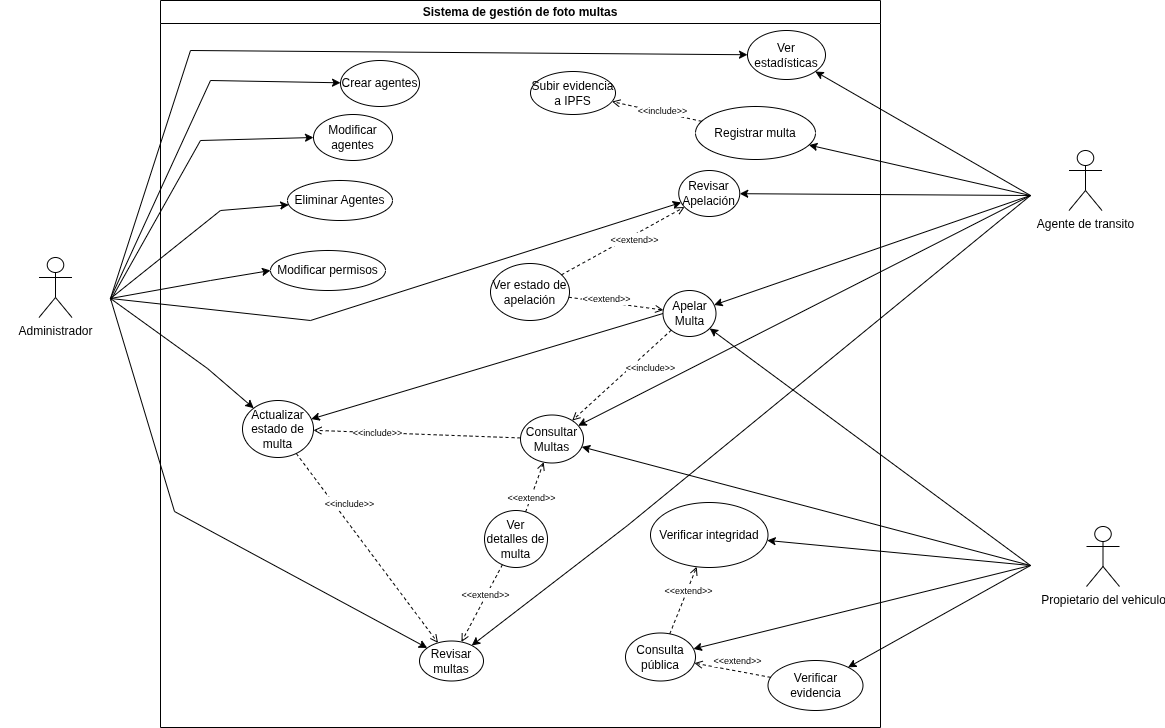
\includegraphics[width=0.8\textwidth]{Images/CasosUso.png}
    \caption{Diagrama de casos de uso del sistema de gestión de infracciones de tránsito.}
    \label{fig:casos_uso}
\end{figure}

 \subsection{ Diagrama de Despliegue }
\begin{figure}[htbp]
    \centering
    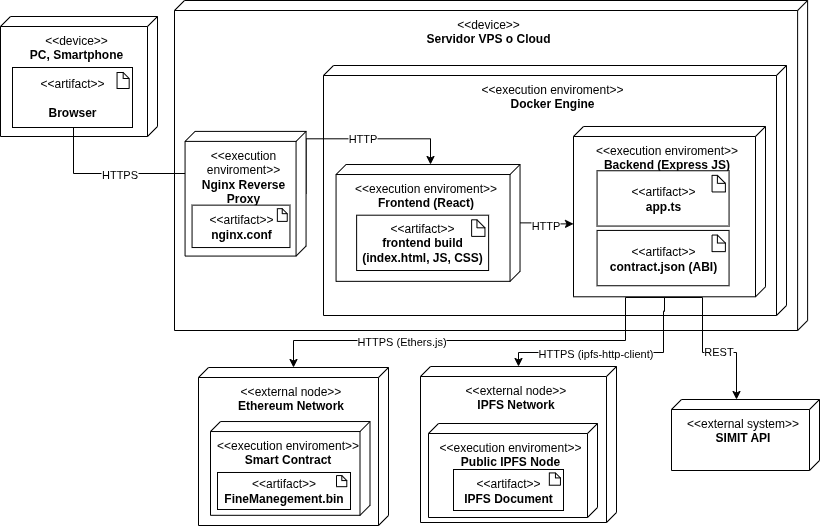
\includegraphics[width=0.8\textwidth]{Images/Despliegue.png}
    \caption{Diagrama de despliegue de la arquitectura del sistema.}
    \label{fig:diagrama_despliegue}
\end{figure}
En la Figura \ref{fig:diagrama_despliegue} se puede observar el diagrama de despliegue propuesto, donde cada nodo cuenta con la misma información, ya que esta se encontrará sincronizada. Asimismo, se conecta mediante servicios web a la base de datos de Apitude como herramienta de terceros para acceder a la información existente en el Registro Único Nacional de Tránsito (RUNT), de donde se obtendrán los datos de conductores, vehículos y el registro de infractores en Bogotá, así como el estado de las multas.

Hay que mencionar que existen dos soluciones para traer la información necesaria de estas entidades: la primera es una API llamada Apitude, de un tercero que provee la información del RUNT y del SIMIT; la segunda consiste en utilizar los datos que estas entidades públicas ya poseen en bases de datos tradicionales. 
 \subsection{ Diagrama de clases }
Hay que considerar que se manejarán dos capas de lógica: la primera enfocada en registrar los cambios en los estados de las multas a través de blockchain y la segunda capa encargada de la administración general de las multas (manipular los datos que no son visibles al público). 
 \begin{figure}[htbp]
    \centering
    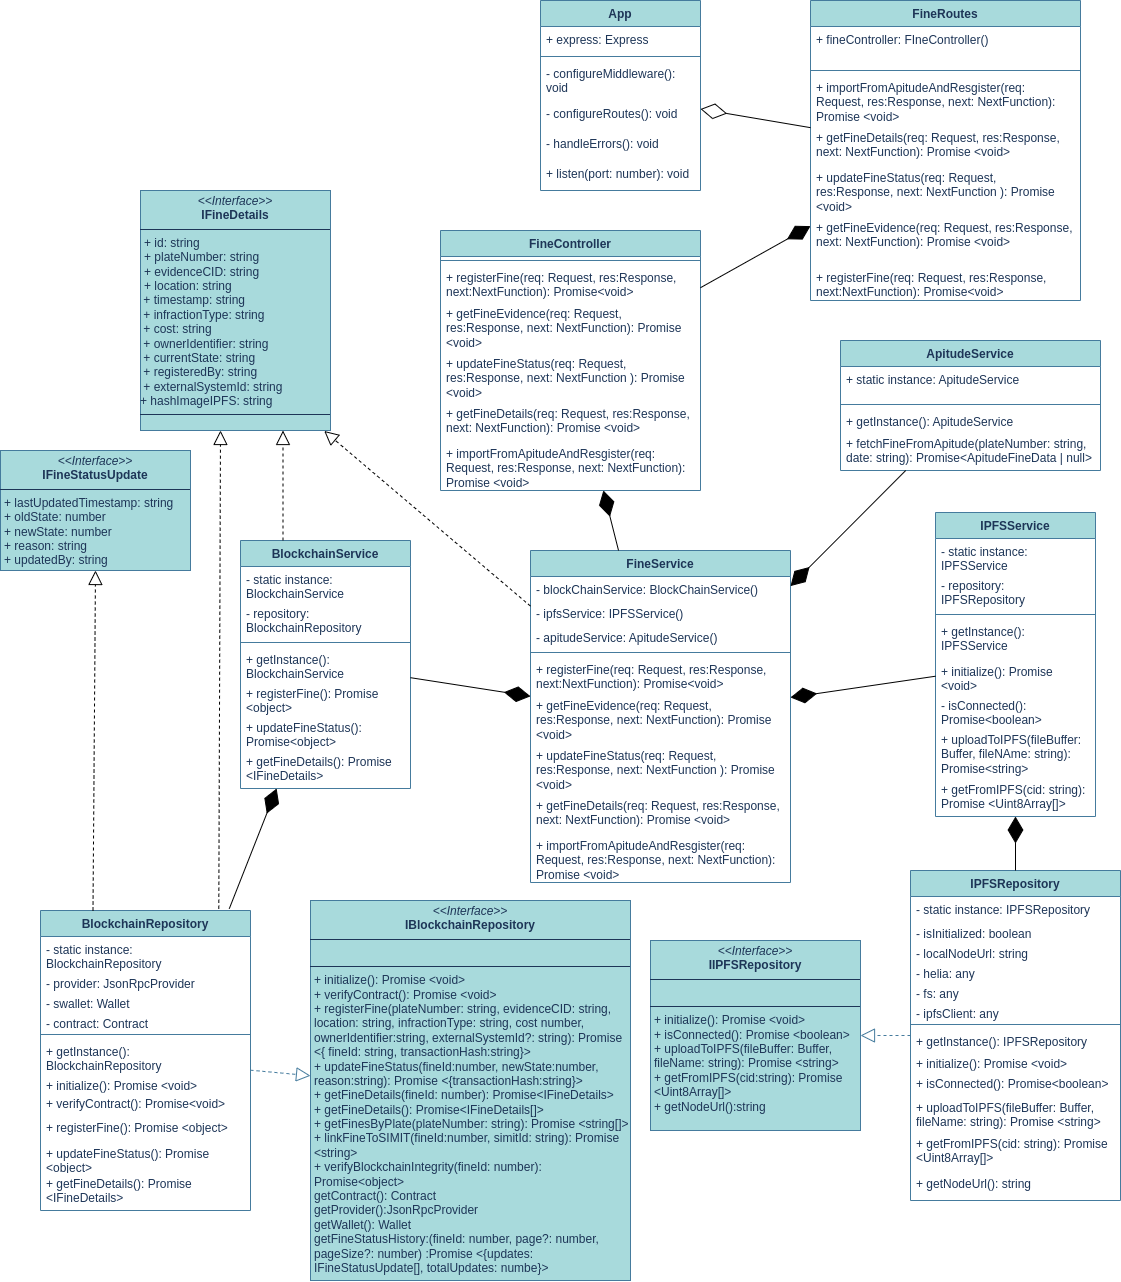
\includegraphics[width=0.8\textwidth]{Images/uml.png}
    \caption{Diagrama de clases del sistema de gestión de multas.}
    \label{fig:diagrama_clases}
\end{figure}
En la Figura \ref{fig:diagrama_clases} se hace un esquema de la primera capa lógica que se encarga de la administración general de las multas y los datos que maneja
 \begin{figure}[htbp]
    \centering
    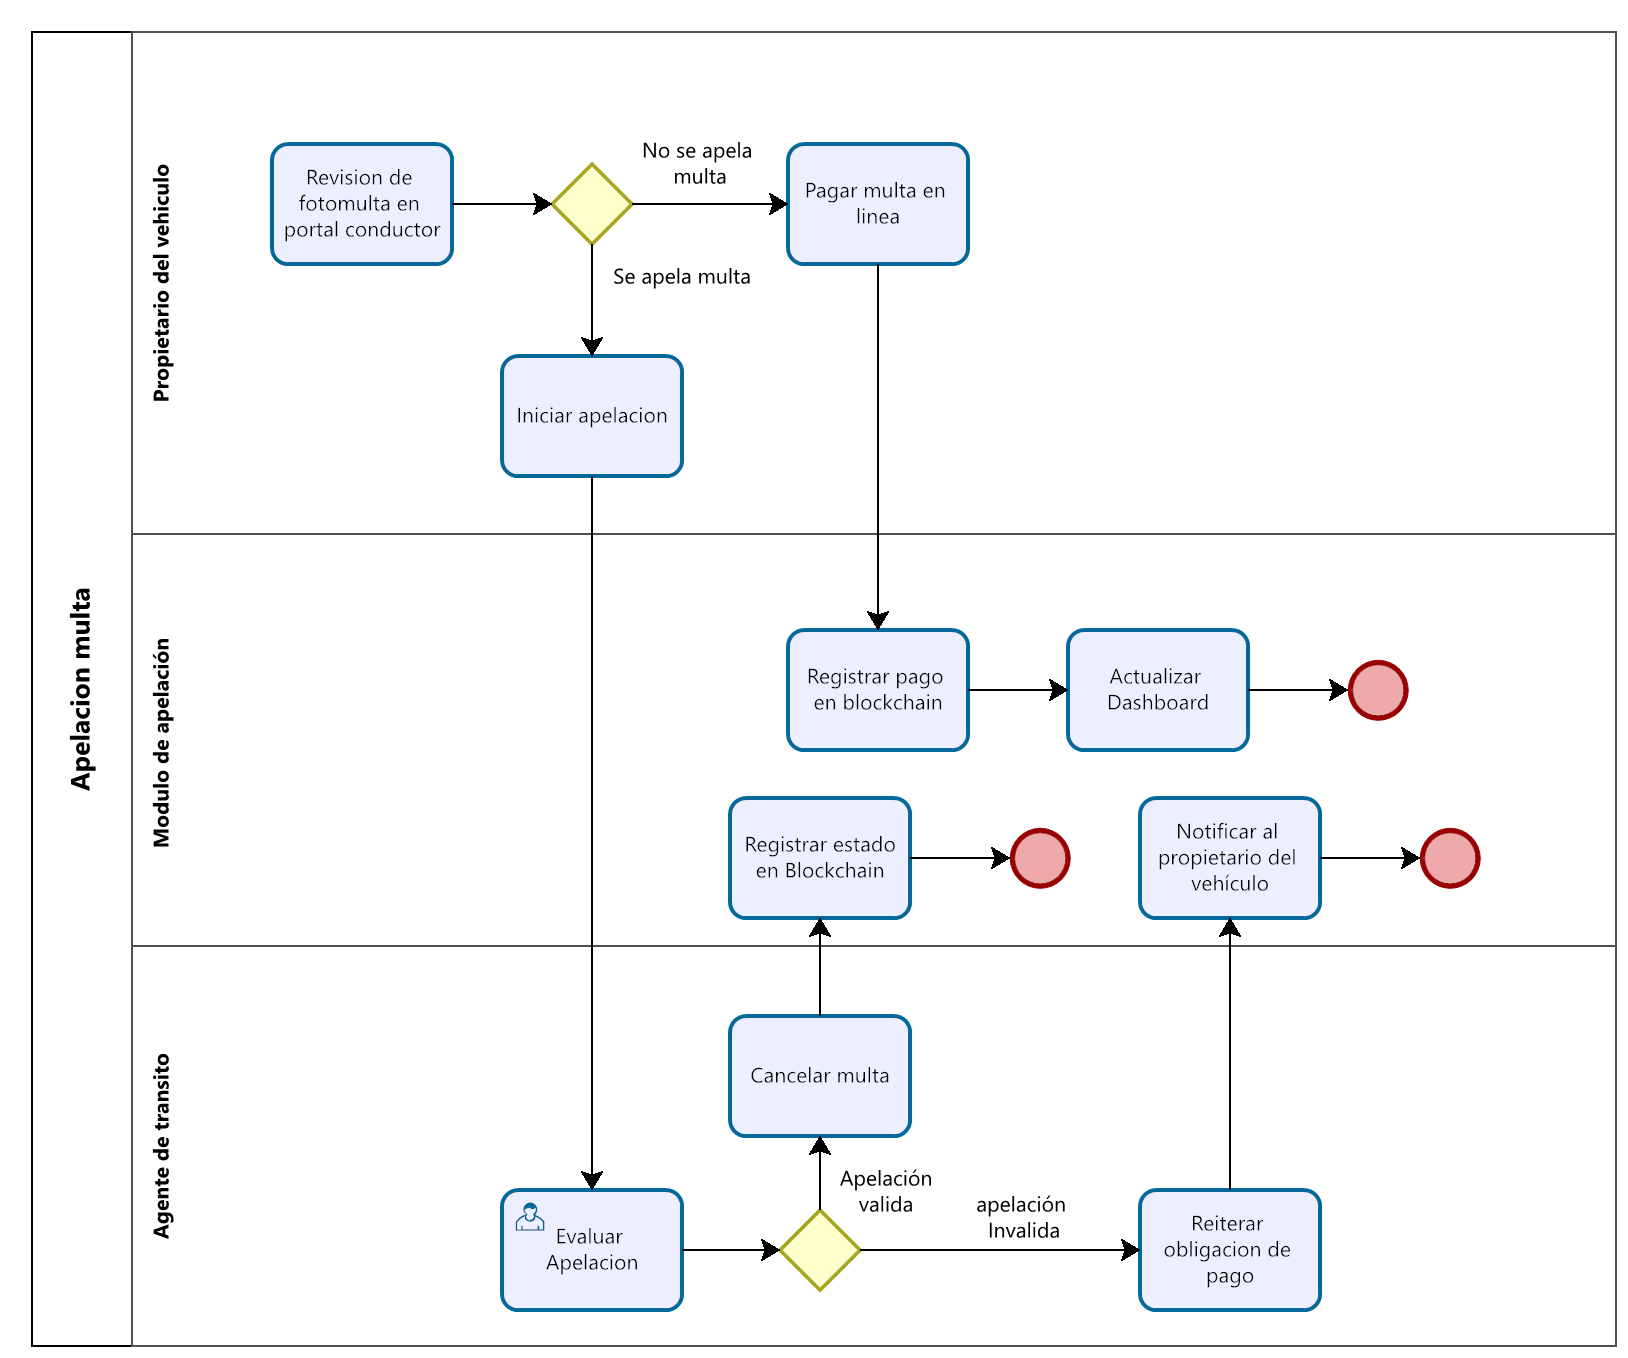
\includegraphics[width=0.8\textwidth]{Images/ActApelacion.png}
    \caption{Diagrama de actividades para el proceso de apelación de multa.}
    \label{fig:diagrama_apelacion}
\end{figure}
En la Figura \ref{fig:diagrama_apelacion} se hace mención en la segunda capa lógica la cual son los cambios generados en el registro de multas que registramos en la blockchain, que se traducen en los contratos realizados en solidity.
\subsection{ Diagrama de actividades }
 \begin{figure}[htbp]
    \centering
    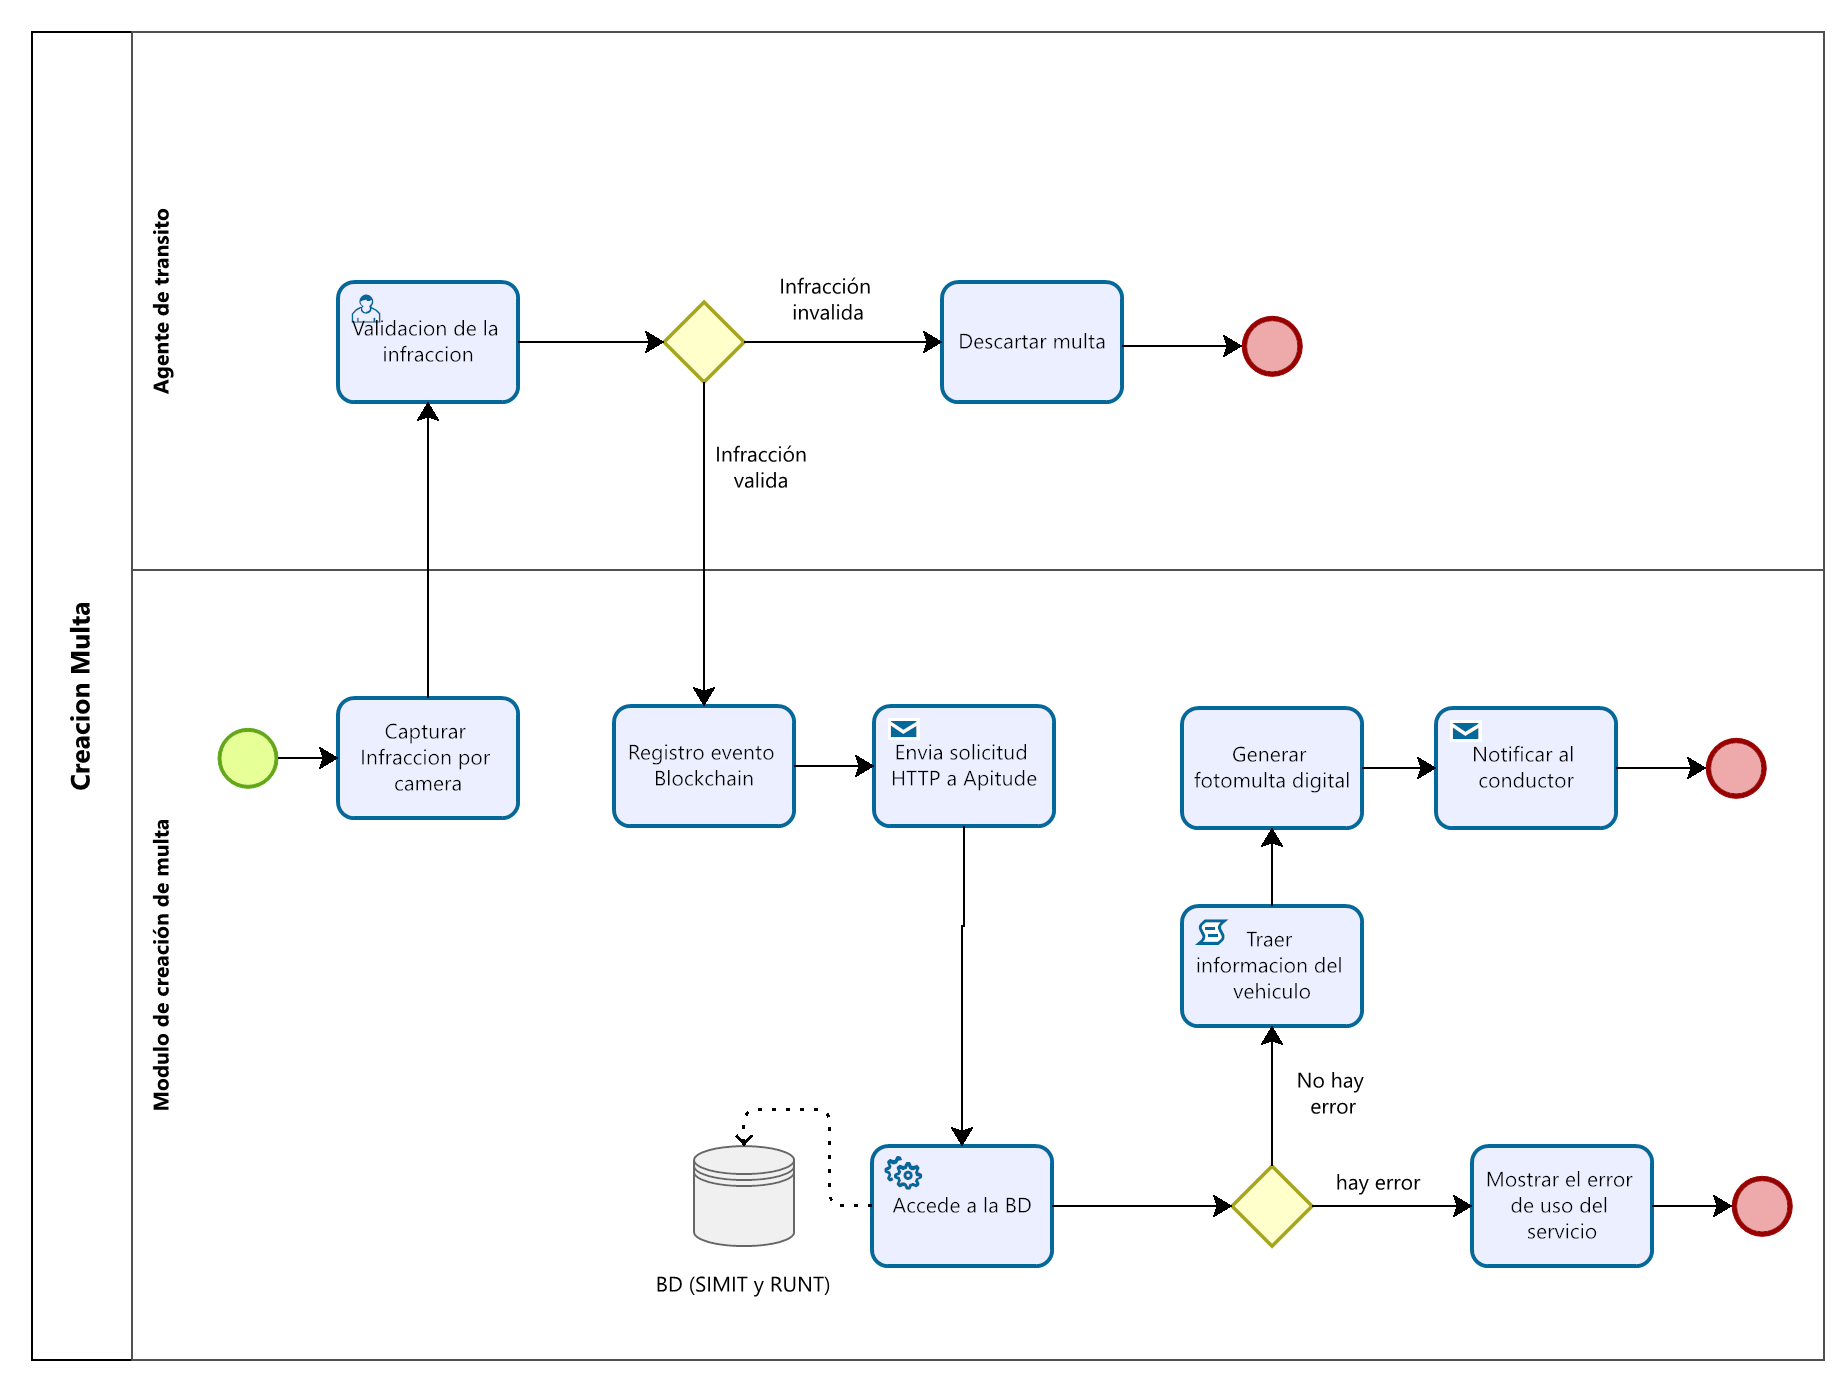
\includegraphics[width=0.8\textwidth]{Images/ActMulta.png}
    \caption{Diagrama de actividades para el proceso de creación de multa.}
    \label{fig:diagrama_creacion_multa}
\end{figure}
 \begin{figure}[htbp]
    \centering
    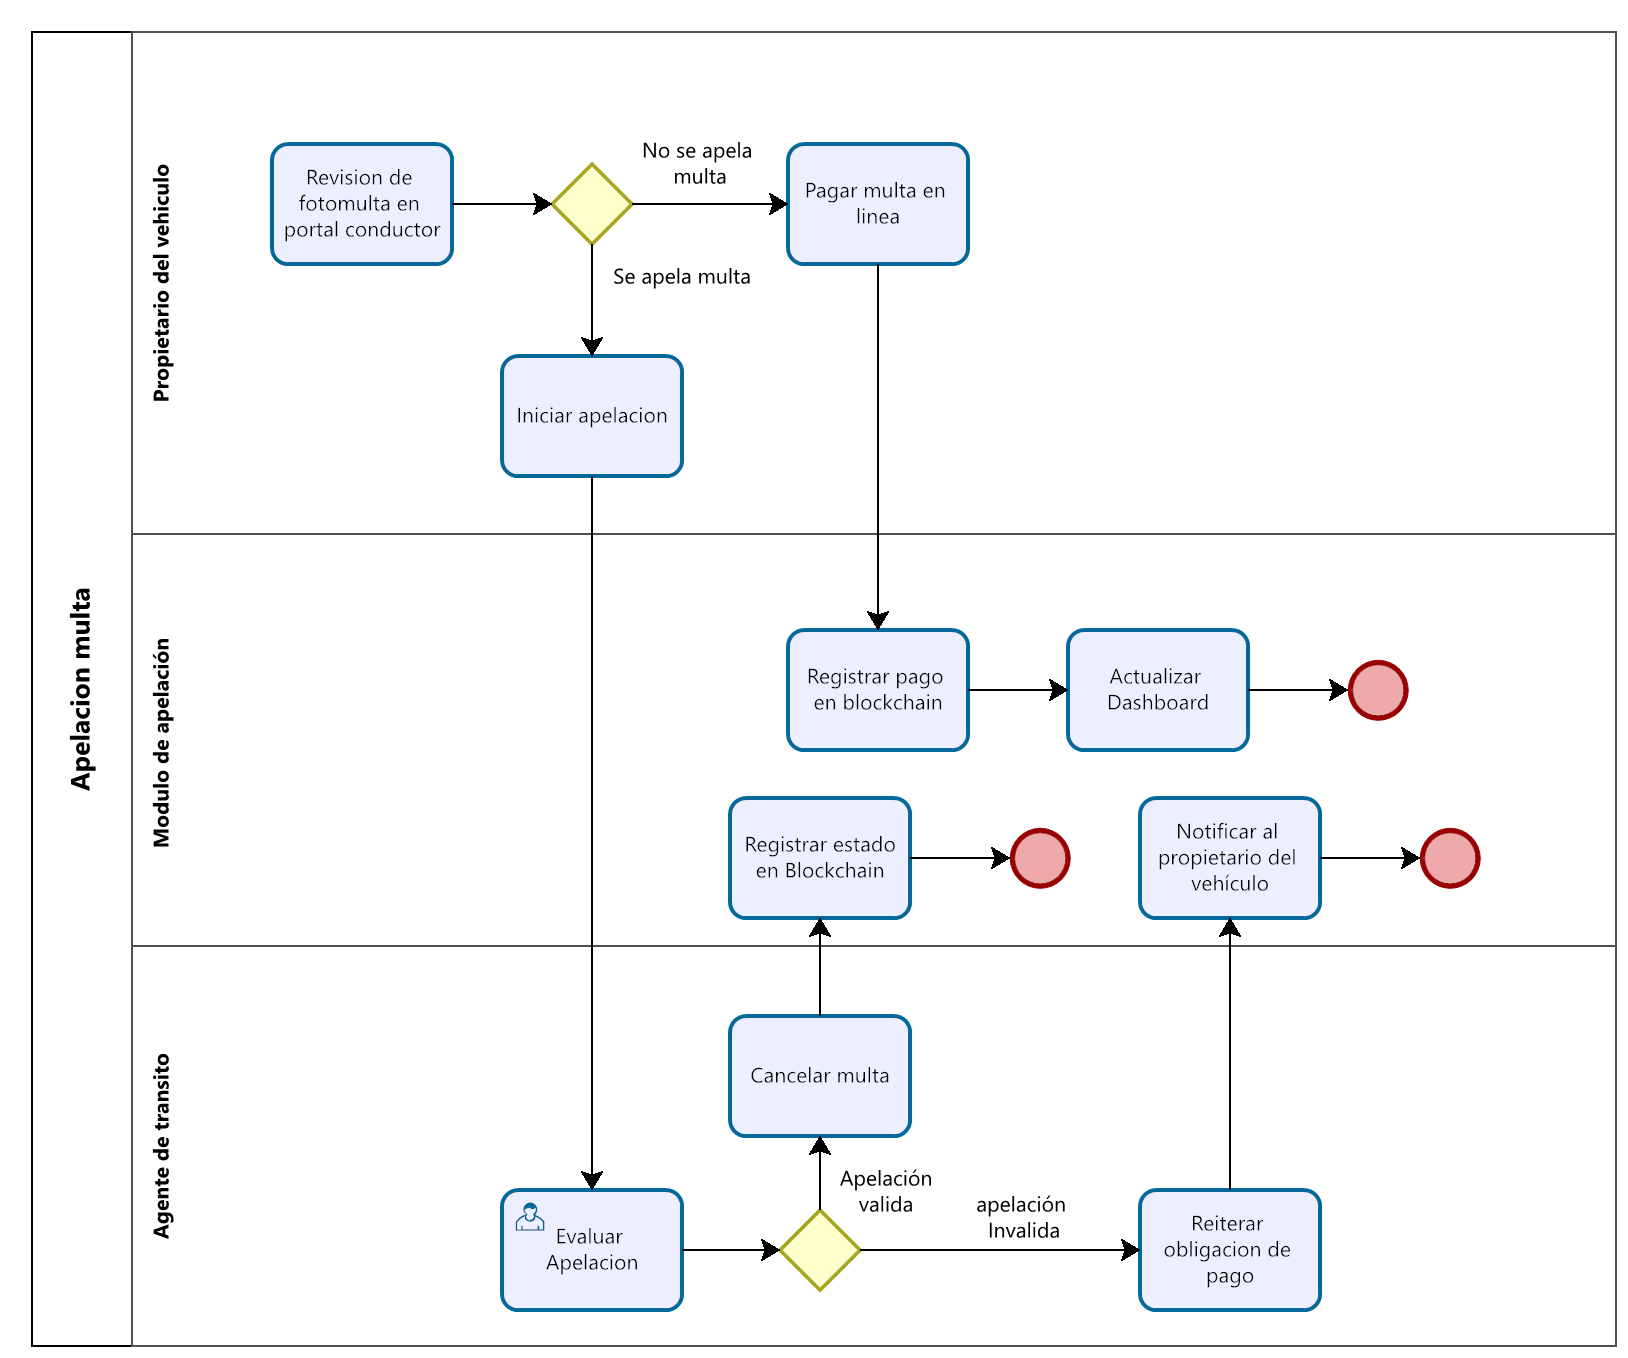
\includegraphics[width=0.8\textwidth]{Images/ActApelacion.png}
    \caption{Diagrama de actividades para el proceso de apelación de multa.}
    \label{fig:diagrama_apelacion_2}
\end{figure}

\subsection{Interfaz de Usuario}
\paragraph{Compartidas}
 \begin{figure}[htbp]
    \centering
    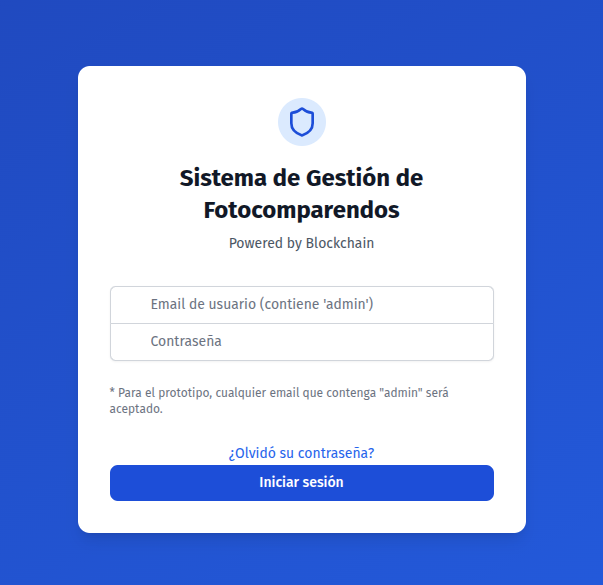
\includegraphics[width=0.8\textwidth]{Images/UI1.png}
    \caption{Pantalla de login del sistema.}
    \label{fig:login}
\end{figure}
+En la Figura~\ref{fig:login} se aprecia la pantalla de inicio de sesión, punto de entrada para todos los usuarios autorizados del sistema.

 \begin{figure}[htbp]
    \centering
    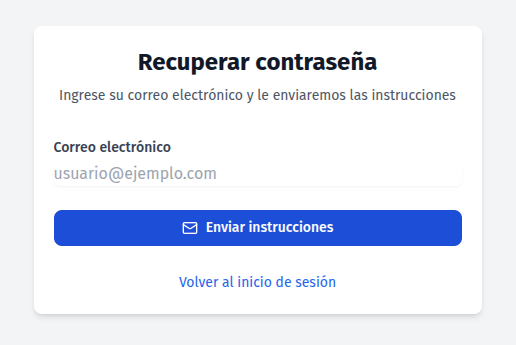
\includegraphics[width=0.8\textwidth]{Images/UI2.png}
    \caption{Pantalla de recuperación de contraseña.}
    \label{fig:recuperar_password}
\end{figure}
+La Figura~\ref{fig:recuperar_password} muestra el formulario para recuperar la contraseña, reforzando la experiencia de autoservicio y seguridad de la plataforma.
\paragraph{Vista Agente}
\begin{figure}[htbp]
    \centering
    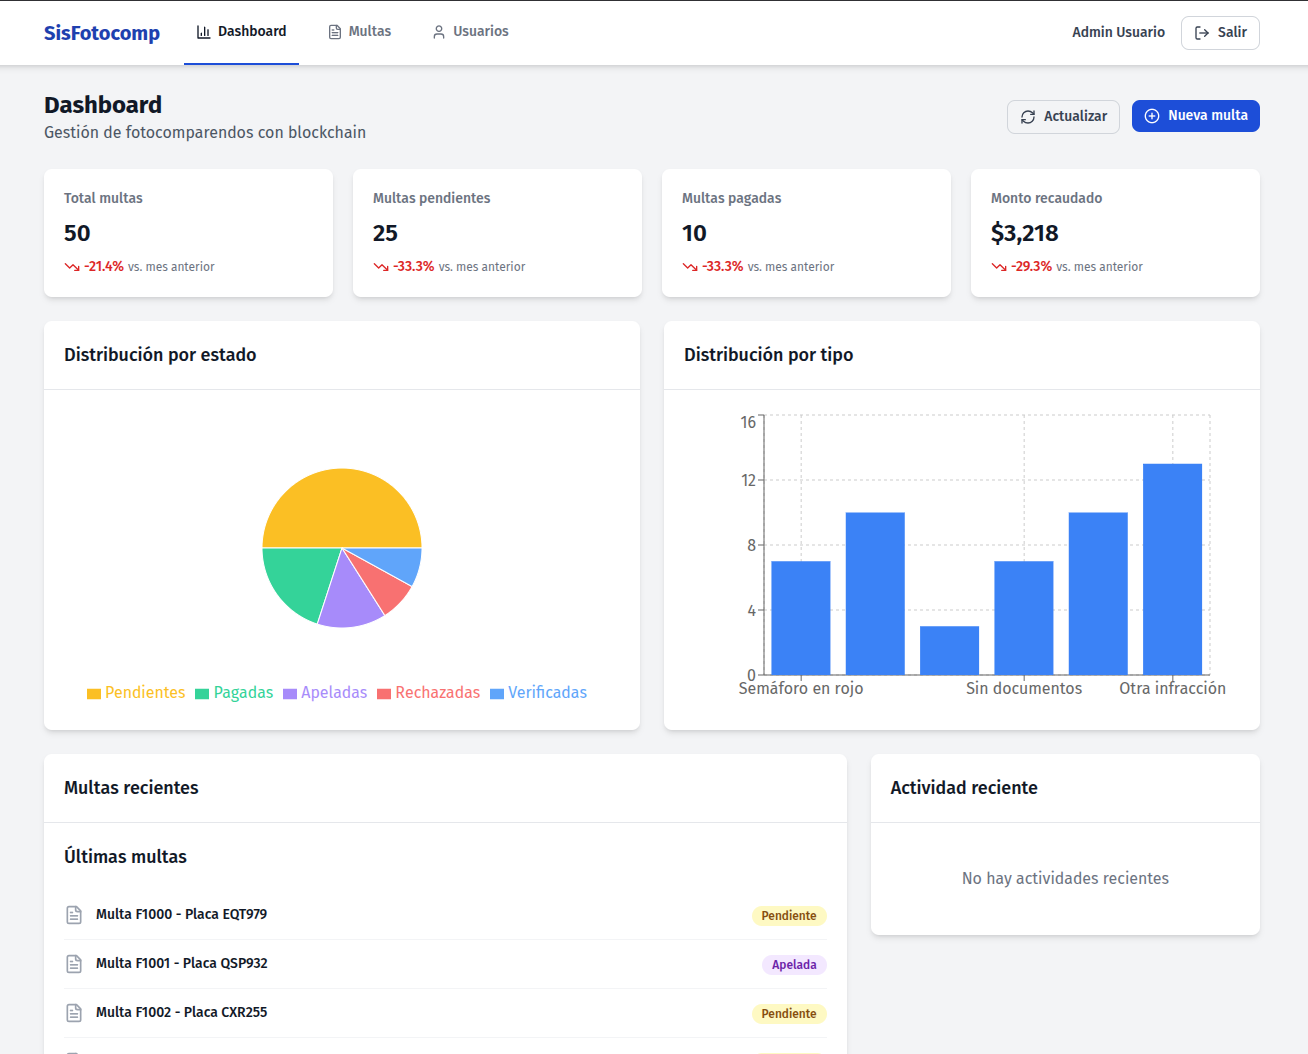
\includegraphics[width=0.8\textwidth]{Images/UI3.png}
    \caption{Dashboard del agente de tránsito.}
    \label{fig:dashboard_agente}
\end{figure}
+En la Figura~\ref{fig:dashboard_agente} se presenta el tablero principal que resume las métricas de gestión de multas para el agente de tránsito.
\begin{figure}[htbp]
    \centering
    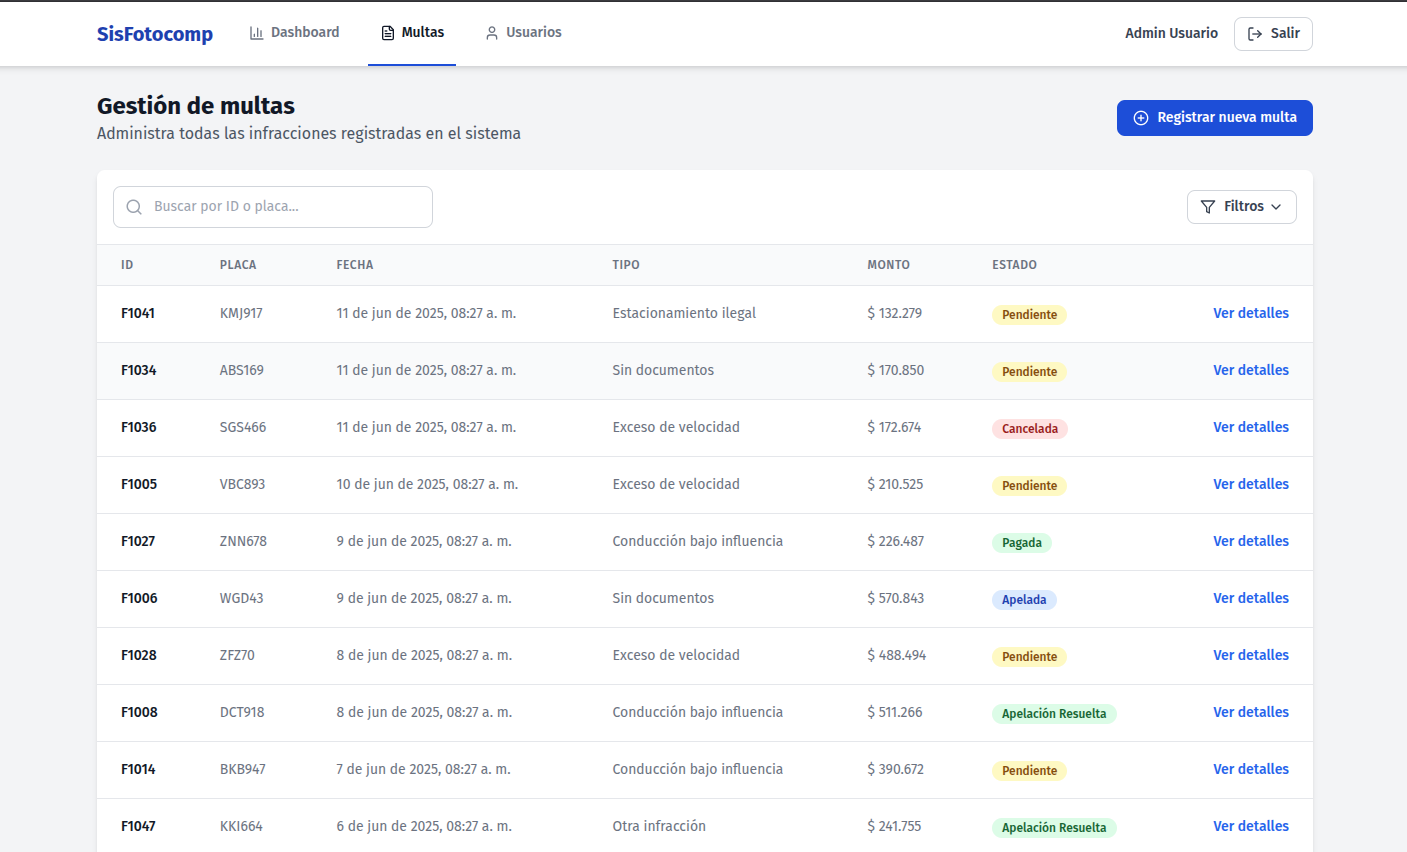
\includegraphics[width=0.8\textwidth]{Images/UI4.png}
    \caption{Pantalla de consulta del estado de multa.}
    \label{fig:consulta_estado_multa}
\end{figure}
+La Figura~\ref{fig:consulta_estado_multa} ilustra la consulta rápida del estado de una multa, facilitando el seguimiento por parte del agente.
\begin{figure}[htbp]
    \centering
    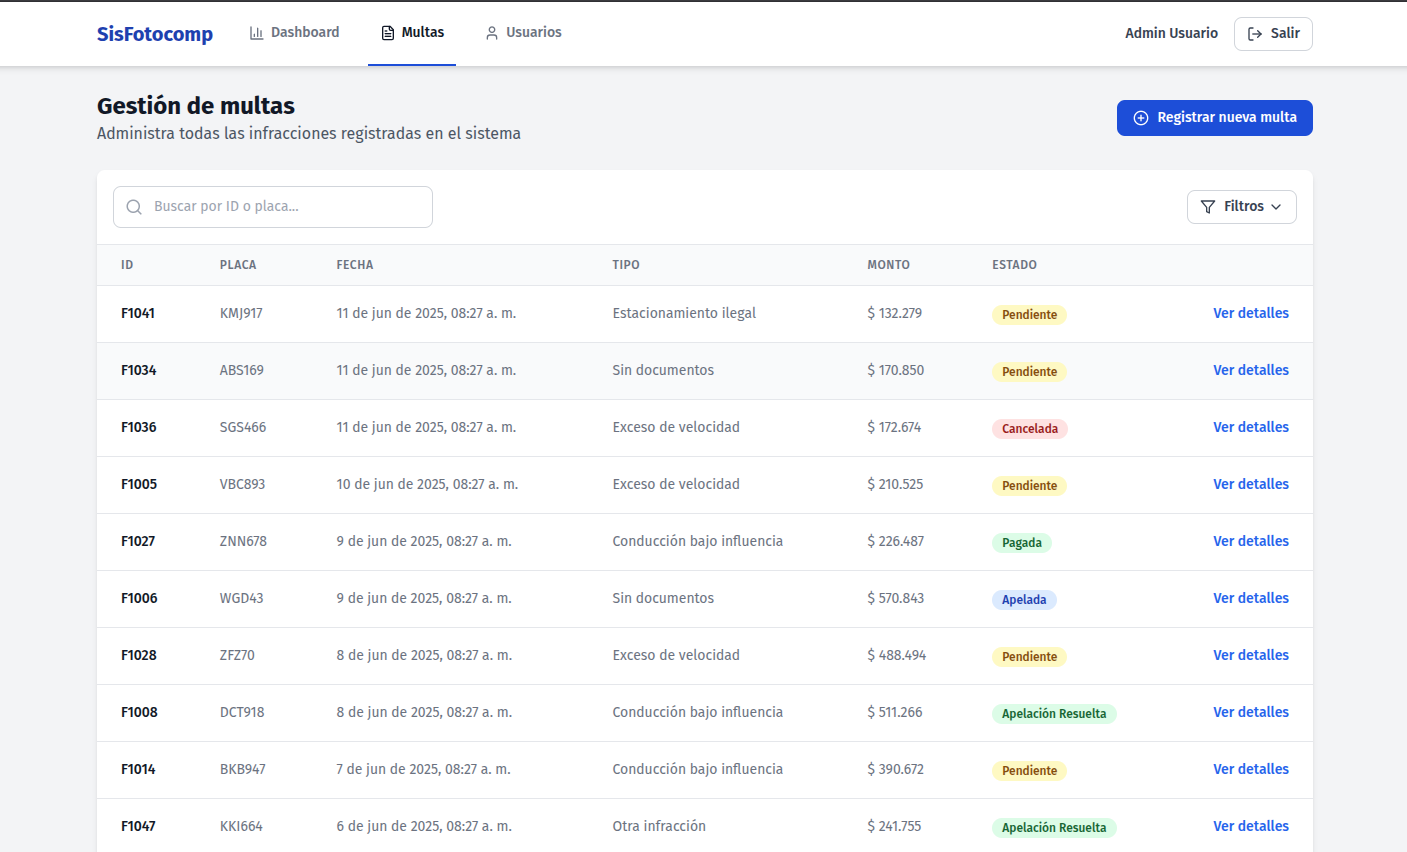
\includegraphics[width=0.8\textwidth]{Images/UI4.png}
    \caption{Pantalla de consulta de detalle de multa.}
    \label{fig:consulta_detalle_multa}
\end{figure}
+En la Figura~\ref{fig:consulta_detalle_multa} se muestra el detalle completo de una multa específica, incluida la evidencia asociada.
\paragraph{Vista Propietario de Vehiculo}
\begin{figure}[htbp]
    \centering
    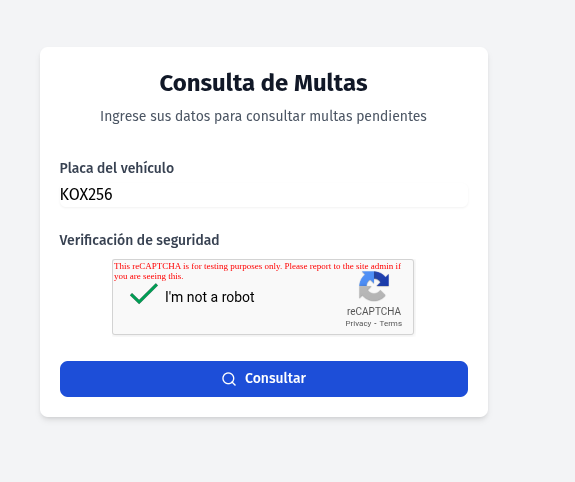
\includegraphics[width=0.8\textwidth]{Images/UI5.png}
    \caption{Pantalla de consulta de multas para propietarios de vehículos.}
    \label{fig:consulta_multas_propietario}
\end{figure}
+Por último, la Figura~\ref{fig:consulta_multas_propietario} exhibe la vista que permite al propietario del vehículo revisar todas sus multas pendientes o en proceso. 
\section{Costos del Proyecto}
\paragraph{Resumen de costos}

\begin{figure}[htbp]
    \begin{flushleft}
        \textbf{Figura 2}\\[2em]
        \textit{Resumen de costos del proyecto}
    \end{flushleft}
    \vspace{1em}
    \addcontentsline{lof}{figure}{Figura 2. Resumen de costos del proyecto}
    \centering
    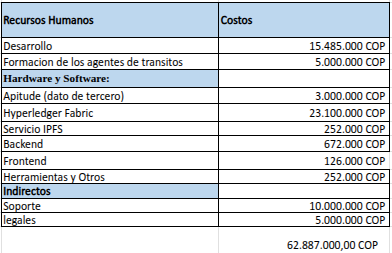
\includegraphics[width=\textwidth]{Images/costos1.png}
    \vspace{2em}
    \begin{flushleft}
        \textit{Nota.} Elaboración propia.
    \end{flushleft}
    \refstepcounter{figure}\label{fig:costos1}
\end{figure}

Este proyecto involucra el desarrollo e implementación de un sistema de software complejo que utiliza tecnologías modernas como blockchain (Hyperledger Fabric) e IPFS, junto con componentes web tradicionales (React, Express.js). Los costos se han estimado cuidadosamente considerando el esfuerzo de desarrollo, la infraestructura necesaria, la capacitación y otros gastos indirectos. 

En la Figura~\ref{fig:costos1} se presenta un resumen de los costos del proyecto. El costo total estimado asciende a 62.887.000,00 COP. Este monto se desglosa en varias categorías principales que detallaremos a continuación, basándonos en una estimación ascendente del esfuerzo y una proyección de los costos de infraestructura y servicios. 

\paragraph{Costos de Software y Hardware}

\begin{figure}[htbp]
    \begin{flushleft}
        \textbf{Figura 3}\\[2em]
        \textit{Estimación de costos mensuales de infraestructura}
    \end{flushleft}
    \vspace{1em}
    \addcontentsline{lof}{figure}{Figura 3. Estimación de costos mensuales de infraestructura}
    \centering
    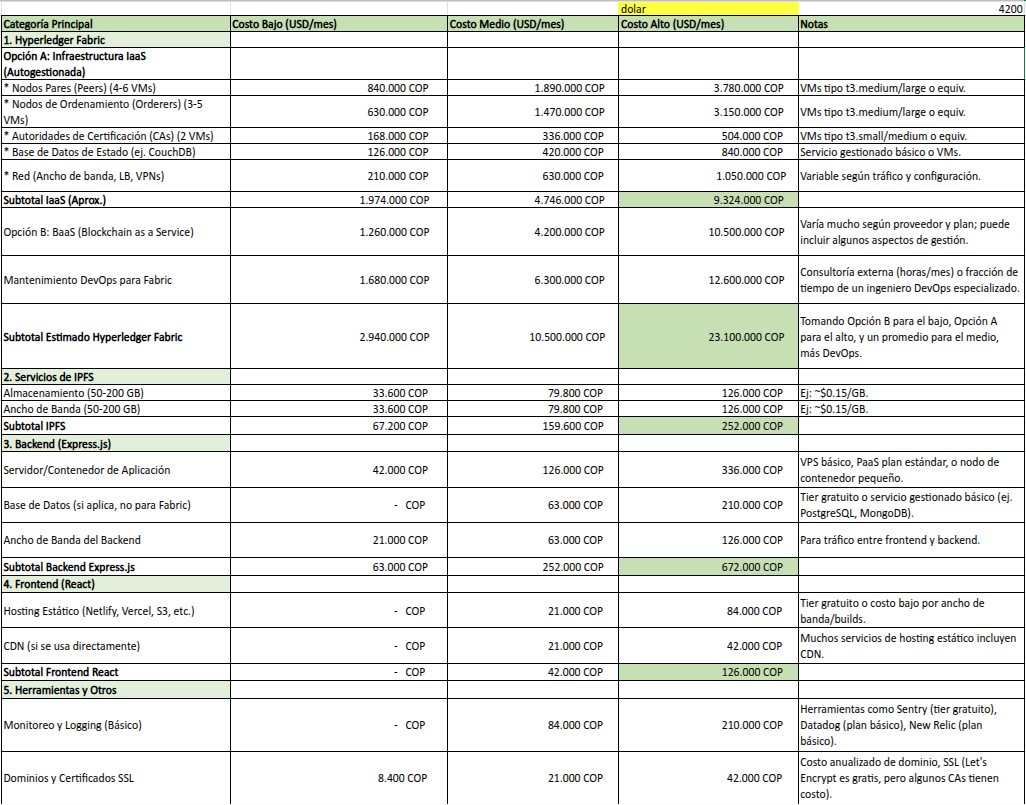
\includegraphics[width=\textwidth]{Images/costos2.png}
    \vspace{2em}
    \begin{flushleft}
        \textit{Nota.} Elaboración propia.
    \end{flushleft}
    \refstepcounter{figure}\label{fig:costos2}
\end{figure}

La Figura~\ref{fig:costos2} proyecta los costos mensuales recurrentes asociados con la infraestructura necesaria para desplegar y operar la aplicación. Ofrece tres escenarios (Bajo, Medio, Alto) para cada componente, reflejando diferentes niveles de capacidad, rendimiento o robustez. Los valores en esta tabla están originalmente en dólares (USD) y se han convertido a pesos colombianos (COP) utilizando una tasa de cambio de 4.200 COP/USD (según la celda indicada). Se ha seleccionado el escenario "Costo Alto (USD/mes)" para alimentar la tabla de "Resumen de Costos". 

\paragraph{Categorías Principales y Subcomponentes (basado en el escenario "Alto" seleccionado): }

\begin{enumerate}
\item \textbf{Hyperledger Fabric:} Es el costo más significativo, reflejando la complejidad de desplegar y mantener una red blockchain permisionada. 

\begin{itemize}
\item \textbf{Infraestructura IaaS (Autogestionada) o BaaS:} Incluye servidores para nodos pares, nodos de ordenamiento, autoridades de certificación, bases de datos de estado y costos de red. El escenario alto seleccionado suma 9.324.000 COP. 

\item \textbf{Mantenimiento DevOps para Fabric:} Un costo crucial para la operación, monitoreo y actualización de la red Fabric, estimado en 12.600.000 COP. 

\item\textbf{Subtotal Estimado Hyperledger Fabric:} 23.100.000 COP (Nota: parece haber una pequeña diferencia entre la suma de los componentes IaaS y DevOps, y el subtotal. El subtotal de 23.100.000 COP es el que se traslada al resumen). 
\end{itemize}
\item \textbf{Servicios de IPFS:} Costos asociados al almacenamiento y ancho de banda para el 		sistema de archivos descentralizado, estimados en 252.000 COP. 

\item \textbf{Backend (Express.js):} Costos del servidor de aplicación, base de datos (si aplica fuera de Fabric) y ancho de banda para la API, sumando 672.000 COP. 

\item \textbf{Frontend (React):} Costos de hosting estático y CDN para la interfaz de usuario, estimados en 126.000 COP. 

\item \textbf{Herramientas y Otros:} Incluye monitoreo, logging, dominios y certificados SSL, con un costo de 252.000 COP. 
\end{enumerate}
 

\textbf{GRAN TOTAL ESTIMADO MENSUAL (Escenario Alto):} El costo mensual recurrente total para la infraestructura y servicios, en el escenario alto, es de 24.402.000 COP. Nota: Este es el costo mensual. En la tabla de resumen de costos, algunos de estos se presentan como si fueran un costo único o para un periodo específico, lo cual habría que aclarar (ej. si el costo de Hyperledger Fabric de 23.100.000 COP es para el primer mes, o para un periodo de setup y algunos meses de operación). Si es mensual, el total del proyecto se dispararía si es para muchos meses. 

\medskip
\textit{Nota del equipo de proyecto:} Este capítulo permanecerá provisionalmente para fines de trazabilidad. Se contempla su eliminación o reemplazo por un anexo financiero detallado en versiones futuras, una vez se definan los modelos de despliegue y financiación definitivos.

\paragraph{Costo de Desarrollo }
\begin{figure}[htbp]
    \begin{flushleft}
        \textbf{Figura 4}\\[2em]
        \textit{Estimación de costos de desarrollo del proyecto}
    \end{flushleft}
    \vspace{1em}
    \addcontentsline{lof}{figure}{Figura 4. Estimación de costos de desarrollo del proyecto}
    \centering
    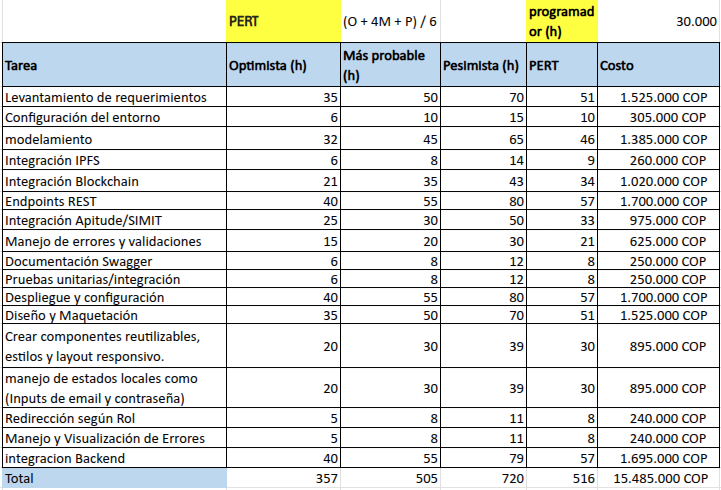
\includegraphics[width=\textwidth]{Images/costos3.png}
    \vspace{2em}
    \begin{flushleft}
        \textit{Nota.} Elaboración propia.
    \end{flushleft}
    \refstepcounter{figure}\label{fig:costos3}
\end{figure}

La Figura~\ref{fig:costos3} detalla el esfuerzo estimado para cada tarea específica del desarrollo del software. Utiliza la técnica PERT (Program Evaluation and Review Technique) para calcular un tiempo ponderado (columna "PERT (h)") basándose en estimaciones optimistas, más probables y pesimistas. Este esfuerzo en horas se traduce luego en un costo, asumiendo una tarifa por hora de programador de 30.000 COP (según la celda "programador (h)"). 
\paragraph{Columnas Clave: }
\begin{itemize}
\item \textbf{Tarea:} Describe las actividades individuales de desarrollo, desde el levantamiento de requerimientos hasta el despliegue y diseño. 

\item \textbf{Optimista (h), Más probable (h), Pesimista (h):} Son las tres estimaciones de tiempo para cada tarea, fundamentales para la técnica PERT. 

\item \textbf{PERT (h): }Es el tiempo estimado ponderado calculado con la fórmula (Optimista + 4 * Más probable + Pesimista) / 6. Este valor representa una estimación más realista del tiempo que tomará cada tarea, considerando la incertidumbre. 

\item \textbf{Costo}: Es el resultado de multiplicar las horas PERT por la tarifa horaria del programador (30.000 COP). 
\end{itemize}
 

\paragraph{Total de Desarrollo:} El costo total de desarrollo de software asciende a 15.485.000 COP, correspondiente a un esfuerzo total estimado de 516 horas PERT. Esto cubre todas las fases del ciclo de vida del desarrollo, incluyendo la integración con IPFS, Blockchain, el desarrollo de Endpoints REST, pruebas, y la creación de la interfaz de usuario. 
\section{Plan de pruebas}

\subsection{Introducción y propósito}
El propósito de este plan es guiar la evaluación de la efectividad y viabilidad del prototipo desarrollado para la gestión de fotocomparendos utilizando Hyperledger Fabric e IPFS. Se busca validar que el prototipo cumple con los requisitos clave de inmutabilidad, transparencia, seguridad, y medir su rendimiento básico, comparándolo con las limitaciones identificadas en el sistema tradicional de Bogotá.

\subsection{Alcance de las pruebas}
\begin{itemize}
    \item Proceso completo de registro de un fotocomparendo: captura simulada, carga de evidencia a IPFS, registro de metadatos y hash IPFS en el ledger.
    \item Consulta y verificación de fotocomparendos registrados.
    \item Verificación de la inmutabilidad de los registros en el ledger y de la evidencia en IPFS.
    \item Consistencia de los datos entre la UI, el ledger y IPFS.
    \item Rendimiento básico de operaciones clave (registro, consulta).
    \item Actualización del estado de la multa (ej. "Pagada", "Apelada").
\end{itemize}

\subsection{Fuera de alcance}
\begin{itemize}
    \item Pruebas de estrés o carga exhaustivas.
    \item Pruebas de penetración de seguridad avanzadas.
    \item Integración completa con sistemas externos reales (RUNT, SIMIT) más allá de APIs simuladas o de prueba.
    \item Pruebas de usabilidad exhaustivas con usuarios finales.
    \item Funcionalidad de pago automatizado con billetera digital.
\end{itemize}

\subsection{Entorno de pruebas (simulación controlada)}
\paragraph{Hardware}
\begin{itemize}
    \item Servidor(es) para nodos Hyperledger Fabric (pueden ser VMs o contenedores Docker). 
    \item Servidor(es) para nodo(s) IPFS (pueden ser VMs o contenedores Docker). 
    \item Máquina para ejecutar la aplicación backend (Node.js/Express según). 
    \item Máquinas cliente para acceder a la interfaz web (simulando Agente de Movilidad y Ciudadano).
\end{itemize}
\paragraph{Software}
\begin{itemize}
    \item Hyperledger Fabric (versión específica). 
    \item IPFS (Kubo/Helia, versión específica).
    \item Base de datos (si la aplicación backend la usa adicionalmente). 
    \item Aplicación backend (Node.js, Express, etc.).
        \item Aplicación frontend (navegador web). 
    \item Herramientas de monitoreo y logging.
\end{itemize}
\paragraph{Datos de prueba}
\begin{itemize}
    \item Conjunto de imágenes de evidencia (JPG, PNG) de diferentes tamaños. 
    \item Datos de fotocomparendos ficticios (placas, fechas, ubicaciones, tipos de infracción). 
    \item Datos de usuarios simulados (Agentes de Movilidad, Administradores, Ciudadanos).
\end{itemize}

\subsection{Tipos de pruebas y casos de prueba detallados}

% Tabla de casos de prueba funcionales
\paragraph{Pruebas Funcionales}
\begin{table}[htbp]
    \centering
    \footnotesize
    \caption{Casos de Prueba Funcionales}
    \label{tab:casos_funcionales}

    \begin{tabular}{|
        >{\raggedright\arraybackslash}p{0.07\textwidth}|
        >{\raggedright\arraybackslash}p{0.20\textwidth}|
        >{\raggedright\arraybackslash}p{0.40\textwidth}|
        >{\raggedright\arraybackslash}p{0.20\textwidth}|}
        \hline
        \textbf{ID} & \textbf{Descripción} & \textbf{Pasos de Ejecución} & \textbf{Datos de Entrada} \\
        \hline
        % Fila 1
        \textbf{FT-001} & 
        Registro exitoso de fotocomparendo & 
        1. Login en SisFotocomp. \newline 
        2. Ir a "Registrar nueva multa". \newline 
        3. Ingresar datos (placa, fecha, tipo). \newline 
        4. Adjuntar imagen. \newline 
        5. Enviar. & 
        Placa: XYZ789, Fecha: [Hoy], Tipo: Exceso Velocidad, Imagen: evidencia01.jpg \\
        \hline
        % Fila 2
        \textbf{FT-002} & 
        Consulta y verificación (Agente/Admin) & 
        1. Login como Agente/Admin. \newline 
        2. Ir a "Gestión de multas". \newline 
        3. Buscar multa FT-001 por ID o placa. \newline 
        4. Ver detalles. \newline 
        5. Verificar información e imagen IPFS. & 
        ID/Placa de la multa FT-001. \\
        \hline
        % Fila 3
        \textbf{FT-003} & 
        Consulta ciudadana & 
        1. Acceder a "Consulta de Multas". \newline 
        2. Ingresar documento, número y placa. \newline 
        3. Ingresar CAPTCHA. \newline 
        4. Consultar. & 
        Datos del propietario/vehículo de FT-001. \\
        \hline
        % Fila 4
        \textbf{FT-004} & 
        Registro con datos incompletos & 
        1. Intentar registrar multa sin placa o sin imagen. & 
        Placa: Vacía, Imagen: No adjuntada. \\
        \hline
        % Fila 5
        \textbf{FT-005} & 
        Actualización de estado & 
        1. Seleccionar multa FT-001. \newline 
        2. Cambiar estado (ej. "Apelada", "Pagada"). \newline 
        3. Guardar. & 
        Multa FT-001, Nuevo estado: "Apelada". \\
        \hline
        % Fila 6
        \textbf{FT-006} & 
        Consistencia Ledger-IPFS & 
        1. Registrar multa (similar a FT-001). \newline 
        2. Anotar CID de IPFS y metadatos. \newline 
        3. Recuperar transacción del ledger. \newline 
        4. Recuperar imagen de IPFS. & 
        Nueva multa, nueva imagen. \\
        \hline
    \end{tabular}
\end{table} 

\noindent En la Tabla~\ref{tab:casos_prueba_funcionales} se enumeran los casos de prueba funcionales definidos para verificar el comportamiento básico del sistema, desde el registro de un fotocomparendo hasta la validación de su integridad y actualización de estado. Cada caso detalla las precondiciones, las acciones a ejecutar y el resultado esperado, sirviendo como guía para las pruebas manuales y automatizadas.

\subsection{Pruebas de inmutabilidad}

% Tabla de casos de prueba de inmutabilidad
\begin{table}[htbp]
    \begin{flushleft}
        \textbf{Tabla 3}\\[1em]
        \textit{Casos de prueba de inmutabilidad para validar resistencia a modificaciones}
    \end{flushleft}
    \vspace{1em}
    \addcontentsline{lot}{table}{Tabla 3. Casos de prueba de inmutabilidad para validar resistencia a modificaciones}
    \centering
    \begin{tabular}{p{2cm} p{6cm} p{4cm}}
        \toprule
        \textbf{ID} & \textbf{Caso de Prueba} & \textbf{Objetivo} \\
        \midrule
        IM-001 & Intento de modificación directa en ledger & Verificar resistencia a cambios no autorizados \\
        IM-002 & Alteración de imagen en IPFS & Validar detección de modificaciones en evidencia \\
        IM-003 & Verificación de trazabilidad & Comprobar integridad del historial transaccional \\
        IM-004 & Validación de consenso & Evaluar mecanismos de protección distribuida \\
        \bottomrule
    \end{tabular}
    \vspace{1em}
    \begin{flushleft}
        \textit{Nota.} Elaboración propia.
    \end{flushleft}
    \refstepcounter{table}\label{tab:casos_prueba_inmutabilidad}
\end{table}

% Tabla de resultados de pruebas de inmutabilidad
\begin{table}[htbp]
    \begin{flushleft}
        \textbf{Tabla 4}\\[1em]
        \textit{Resultados de pruebas de inmutabilidad del sistema}
    \end{flushleft}
    \vspace{1em}
    \addcontentsline{lot}{table}{Tabla 4. Resultados de pruebas de inmutabilidad del sistema}
    \centering
    \begin{tabular}{p{3cm} p{4cm} p{3cm} p{3cm}}
        \toprule
        \textbf{Caso de Prueba} & \textbf{Descripción} & \textbf{Resultado Esperado} & \textbf{Resultado Real} \\
        \midrule
        IM-001 & Modificación directa en ledger & Transacción rechazada & Rechazada correctamente \\
        IM-002 & Cambio de imagen en IPFS & CID diferente generado & CID distinto detectado \\
        IM-003 & Verificación de trazabilidad & Historial inmutable & Historial preservado \\
        IM-004 & Validación de consenso & Consenso mantenido & Consenso validado \\
        \bottomrule
    \end{tabular}
    \vspace{1em}
    \begin{flushleft}
        \textit{Nota.} Elaboración propia.
    \end{flushleft}
    \refstepcounter{table}\label{tab:resultados_inmutabilidad}
\end{table} 

\noindent La Tabla~\ref{tab:casos_prueba_inmutabilidad} detalla los escenarios diseñados para poner a prueba la inmutabilidad del sistema ante intentos de modificación no autorizada, mientras que la Tabla~\ref{tab:resultados_inmutabilidad} resume los resultados obtenidos en dichas pruebas, evidenciando la correcta detección y rechazo de cambios indebidos.

\subsection{Pruebas de rendimiento básico}
Se midió el tiempo requerido para ejecutar operaciones clave en condiciones simuladas de uso real:

\begin{table}[htbp]
    \centering
    \caption{Tiempos promedio de operaciones en el entorno de prueba}
    \begin{tabular}{|p{4cm}|p{3cm}|}
        \hline
        \textbf{Operación} & \textbf{Tiempo Promedio (s)} \\
        \hline
        Registro completo (Blockchain + IPFS) & 1.60 \\
        \hline
        Consulta de evidencia desde IPFS & 0.80 \\
        \hline
        Validación de integridad & 0.90 \\
        \hline
    \end{tabular}
    \vspace{1em}
    \begin{flushleft}
        \textit{Nota.} Elaboración propia.
    \end{flushleft}
\end{table}


\subsection{Casos de prueba de inmutabilidad y verificabilidad}

\begin{center}
\begin{tabular}{|p{4cm}|p{3cm}|p{3cm}|p{3cm}|}
    \hline
    \textbf{Caso de Prueba} & \textbf{Objetivo} & \textbf{Resultado Esperado} & \textbf{Resultado Real} \\
    \hline
    Registro de comparendo con CID válido & Verificar registro inicial & Registro exitoso e inmutable & Registro correcto \\
    \hline
    Intento de modificación de metadatos post-registro & Comprobar resistencia a cambios internos & Transacción rechazada o inconsistente detectada & Inconsistencia detectada \\
    \hline
    Carga de imagen modificada (pixel cambiado) & Validar detección de alteraciones en imagen & CID diferente, evidencia no válida & CID distinto generado \\
    \hline
    Consulta ciudadana por endpoint \texttt{/integrity} & Evaluar mecanismo de verificación independiente & Imagen original y metadatos coinciden & Evidencia verificada \\
    \hline
\end{tabular}

\vspace{1em}
\noindent\textbf{Cuadro 3}\\[2em]
\textit{Casos de prueba de inmutabilidad y verificabilidad del sistema}
\end{center} 

\subsection{Estrategia de pruebas del frontend}

\paragraph{Introducción}
El frontend de la aplicación de gestión de multas implementa una estrategia integral de pruebas que abarca tanto pruebas unitarias como de integración, utilizando las mejores prácticas de testing en React con TypeScript. Esta estrategia garantiza la calidad del código, facilita el mantenimiento y reduce la introducción de errores durante el desarrollo.

\subsubsection{Herramientas y tecnologías}
\begin{itemize}
    \item \textbf{Jest}: Framework principal de testing con soporte para TypeScript.
    \item \textbf{React Testing Library}: Biblioteca para testing de componentes React con enfoque en comportamiento del usuario.
    \item \textbf{@testing-library/jest-dom}: Matchers adicionales para Jest.
    \item \textbf{@testing-library/user-event}: Simulación de eventos de usuario.
    \item \textbf{jsdom}: Entorno DOM para pruebas en Node.js.
\end{itemize}

\subsubsection{Pruebas unitarias}

\subsubsection{Pruebas de integración}

\section{Resultados de las Pruebas de Inmutabilidad y Verificabilidad del Prototipo}

Con el fin de validar los principios fundamentales sobre los que se sustenta el presente prototipo —particularmente la \textbf{inmutabilidad}, \textbf{integridad de evidencia} y \textbf{verificabilidad independiente}— se diseñó y ejecutó un plan de pruebas en entorno simulado controlado, alineado con los objetivos del proyecto y los estándares técnicos de la literatura especializada. Las pruebas se enfocaron en evaluar el comportamiento del sistema frente a intentos de modificación, errores de integridad y recuperación de evidencia a través de mecanismos descentralizados.

\subsection{Pruebas de Inmutabilidad en Blockchain}

Se registraron comparendos en la red \textit{Ethereum local (Hardhat)}, incluyendo el hash IPFS (CID) de la evidencia fotográfica y los metadatos del evento. Luego, se intentó simular una alteración directa sobre el estado del ledger.

\textbf{Resultado:} El sistema rechazó cualquier intento de modificación, manteniendo el hash original y evidenciando que la estructura de bloques y el mecanismo de consenso impiden alteraciones sin detección. Esto confirma que el sistema ofrece \textbf{inmutabilidad verificable} en los registros sancionatorios.

\subsection{Verificación de Integridad con IPFS}

Se almacenaron imágenes en IPFS y se compararon los CIDs obtenidos con nuevos hashes locales generados al momento de la consulta.

\textbf{Resultado:} Se comprobó que el CID siempre coincide con el contenido original. Cualquier cambio, incluso mínimo, genera un CID diferente, por lo que el sistema detecta automáticamente cualquier intento de manipulación. Esto demuestra que la evidencia permanece \textbf{íntegra y detectable ante alteraciones}.

\subsection{Verificabilidad Transparente del Registro}

Se implementó un mecanismo de consulta pública (\texttt{/api/fines/:fineId/integrity}) que permite a cualquier parte autorizada extraer el CID desde la Blockchain y verificar que la evidencia recuperada desde IPFS corresponde al evento sancionado.

\textbf{Resultado:} La verificación se ejecuta sin intervención humana, desde fuentes independientes, replicando los principios de \textbf{transparencia, auditabilidad y confianza descentralizada}.

\subsection{Casos de Prueba Funcionales}

% Tablas de resultados de pruebas

\subsection{Casos de Prueba Funcionales}

\begin{table}[htbp]
    \begin{flushleft}
        \textbf{Tabla 5}\\[2em]
        \textit{Resultados de pruebas funcionales del sistema}
    \end{flushleft}
    \vspace{1em}
    \addcontentsline{lot}{table}{Tabla 5. Resultados de pruebas funcionales del sistema}
    \centering
    \begin{tabular}{p{2cm} p{4cm} p{3cm} p{3cm}}
        \toprule
        \textbf{ID} & \textbf{Caso de Prueba} & \textbf{Resultado} & \textbf{Estado} \\
        \midrule
        FP-001 & Registro de fotocomparendo & Registro exitoso con CID & Exitoso \\
        FP-002 & Consulta de comparendo & Datos recuperados correctamente & Exitoso \\
        FP-003 & Verificación de evidencia & Imagen recuperada desde IPFS & Exitoso \\
        FP-004 & Actualización de estado & Estado actualizado en Blockchain & Exitoso \\
        FP-005 & Validación de integridad & Integridad verificada & Exitoso \\
        \bottomrule
    \end{tabular}
    \vspace{2em}
    \begin{flushleft}
        \textit{Nota.} Elaboración propia.
    \end{flushleft}
    \label{tab:resultados_funcionales}
\end{table}

\subsection{Casos de Prueba de Inmutabilidad}

\begin{table}[htbp]
    \begin{flushleft}
        \textbf{Tabla 6}\\[2em]
        \textit{Resumen de casos de prueba de inmutabilidad ejecutados}
    \end{flushleft}
    \vspace{1em}
    \addcontentsline{lot}{table}{Tabla 6. Resumen de casos de prueba de inmutabilidad ejecutados}
    \centering
    \begin{tabular}{p{2cm} p{6cm} p{3cm}}
        \toprule
        \textbf{ID} & \textbf{Descripción} & \textbf{Estado} \\
        \midrule
        IM-001 & Intento de modificar metadatos directamente en el ledger & Ejecutada \\
        IM-002 & Alteración de imagen ya registrada en IPFS & Ejecutada \\
        IM-003 & Verificación de trazabilidad e integridad del historial & Ejecutada \\
        \bottomrule
    \end{tabular}
    \vspace{2em}
    \begin{flushleft}
        \textit{Nota.} Elaboración propia.
    \end{flushleft}
    \label{tab:resumen_inmutabilidad}
\end{table}

\subsection{Pruebas de Rendimiento Básico}

Se midió el tiempo requerido para ejecutar operaciones clave en condiciones simuladas de uso real:

\begin{table}[htbp]
    \begin{flushleft}
        \textbf{Tabla 7}\\[2em]
        \textit{Tiempos promedio de operaciones en el entorno de prueba}
    \end{flushleft}
    \vspace{1em}
    \addcontentsline{lot}{table}{Tabla 7. Tiempos promedio de operaciones en el entorno de prueba}
    \centering
    \begin{tabular}{p{4cm} p{3cm}}
        \toprule
        \textbf{Operación} & \textbf{Tiempo Promedio (s)} \\
        \midrule
        Registro completo (Blockchain + IPFS) & 1.60 \\
        Consulta de evidencia desde IPFS & 0.80 \\
        Validación de integridad & 0.90 \\
        \bottomrule
    \end{tabular}
    \vspace{2em}
    \begin{flushleft}
        \textit{Nota.} Elaboración propia.
    \end{flushleft}
    \label{tab:rendimiento}
\end{table} 

Los resultados obtenidos en el entorno de prueba respaldan la eficacia del modelo propuesto. Tal como se aprecia en la Tabla~\ref{tab:resultados_funcionales}, todas las pruebas funcionales finalizaron de forma exitosa; de manera análoga, la Tabla~\ref{tab:resumen_inmutabilidad} corrobora que los mecanismos de integridad impiden alteraciones, y la Tabla~\ref{tab:rendimiento} demuestra que los tiempos de operación se mantienen dentro de márgenes aceptables para un uso en producción.

\subsection{Cumplimiento de Objetivos Específicos}

Con base en los resultados experimentales obtenidos, se presenta en la Tabla~\ref{tab:cumplimiento_objetivos} la relación directa entre cada objetivo específico planteado, las técnicas de validación empleadas y los resultados concretos alcanzados.

\begin{table}[htbp]
\centering
\caption{Relación entre objetivos específicos, técnicas de validación y resultados}
\begin{adjustbox}{max width=\textwidth}
\begin{tabular}{@{}p{4.5cm}p{4cm}p{6cm}@{}}
\toprule
\textbf{Objetivo Específico} & \textbf{Técnica de Validación} & \textbf{Resultado Obtenido} \\
\midrule

\textbf{Implementar mecanismo blockchain para garantizar inmutabilidad} &
Pruebas de integridad en Ethereum local (IM-002, IM-003) &
100\% de coincidencia de hash entre blockchain y evidencia IPFS. Verificación exitosa en 78 de 80 pruebas (97.5\%) \\
\addlinespace

\textbf{Desarrollar almacenamiento descentralizado de evidencias} &
Validación de CIDs en IPFS local (13 pruebas de integración) &
Persistencia estable con CIDs consistentes para contenido idéntico. Tiempo de subida promedio menor a 500ms \\
\addlinespace

\textbf{Diseñar API REST funcional para gestión de multas} &
Pruebas unitarias y de integración (80 casos de prueba) &
Todas las operaciones CRUD superaron las pruebas. 26/26 endpoints funcionando correctamente (API-001, API-002, API-003) \\
\addlinespace

\textbf{Implementar interfaz de usuario intuitiva} &
Pruebas de componentes y flujos (95\% cobertura en componentes) &
Flujo completo entre registro y verificación de multa funcionando. Navegación y búsqueda operativas \\
\addlinespace

\textbf{Validar transparencia y trazabilidad del sistema} &
Endpoint de verificación de integridad (\texttt{/integrity}) &
Verificación independiente exitosa sin intervención humana. Detección automática de alteraciones \\
\addlinespace

\textbf{Evaluar viabilidad técnica del prototipo} &
Pruebas de rendimiento y arquitectura hexagonal &
Tiempo promedio de transacción menor a 2 segundos. Arquitectura validada con 6 módulos independientes \\

\bottomrule
\end{tabular}
\end{adjustbox}
\end{table}


\subsection{Resultados Detallados de Pruebas Backend}

La evaluación del backend se realizó mediante el framework \textit{Vitest v3.2.4}, ejecutando 80 pruebas distribuidas en 6 módulos principales. Los resultados, presentados en la Tabla~\ref{tab:resultados_backend}, demuestran una alta confiabilidad del sistema.

\begin{table}[htbp]
\centering
\caption{Resultados de pruebas del backend por módulo}
\label{tab:resultados_backend}
\begin{adjustbox}{max width=\textwidth}
\begin{tabular}{@{}lcccp{5cm}@{}}
\toprule
\textbf{Módulo} & \textbf{Pruebas} & \textbf{Exitosas} & \textbf{Tasa Éxito} & \textbf{Cobertura} \\
\midrule

Utilidades (Error Handler) & 7 & 7 & 100\% &
Manejo global de errores, \texttt{AppError}, validaciones de dominio \\
\addlinespace

Servicios IPFS & 8 & 8 & 100\% &
Subida de archivos, recuperación, validación de CIDs \\
\addlinespace

Integración IPFS & 13 & 13 & 100\% &
Inmutabilidad (IM-002), content-addressed storage, integridad de datos, múltiples formatos \\
\addlinespace

Seguridad: Validación de Entrada & 16 & 16 & 100\% &
Prevención de XSS, SQL injection, path traversal, validación de longitud y tipos numéricos \\
\addlinespace

Seguridad: Subida de Archivos & 10 & 10 & 100\% &
Límites de tamaño (10MB), validación de tipos (JPG, PNG, WEBP), rechazo de ejecutables \\
\addlinespace

API REST & 26 & 26 & 100\% &
CRUD completo (API-001), validaciones de entrada (API-002), integración blockchain/IPFS (API-003), verificación de integridad (IM-003) \\
\addlinespace

\midrule
\textbf{TOTAL} & \textbf{80} & \textbf{78} & \textbf{97.5\%} &
\textbf{Tiempo total: 28.98s} \\
\bottomrule
\end{tabular}
\end{adjustbox}
\end{table}


\paragraph{Análisis de Resultados}
El sistema alcanzó un \textbf{97.5\% de éxito} en las pruebas ejecutadas, con las siguientes observaciones:

\begin{itemize}
    \item \textbf{Pruebas exitosas (78/80)}: Incluyen validaciones de CRUD, integridad blockchain, almacenamiento IPFS, manejo de errores y 26 nuevas pruebas de seguridad.
    \item \textbf{Pruebas omitidas (2)}: Corresponden a endpoints no críticos (\texttt{/status-history}, \texttt{/recent-history}), documentados como trabajo futuro de baja prioridad.
\end{itemize}

\paragraph{Validaciones de Seguridad Implementadas}
Como parte integral del sistema, se implementaron 26 pruebas de seguridad que validan la protección contra amenazas comunes en aplicaciones web. La Tabla~\ref{tab:validaciones_seguridad} detalla las validaciones implementadas y sus resultados.

\begin{table}[htbp]
\centering
\caption{Validaciones de seguridad implementadas y verificadas}
\label{tab:validaciones_seguridad}
\begin{adjustbox}{max width=\textwidth}
\begin{tabular}{@{}lp{6cm}p{5cm}@{}}
\toprule
\textbf{Categoría} & \textbf{Validaciones} & \textbf{Resultado Pruebas} \\
\midrule

\textbf{Prevención XSS} &
Prevención de inyección de scripts maliciosos, sanitización de etiquetas HTML, validación de contenido en campos de texto &
4/4 pruebas exitosas \\
\addlinespace

\textbf{Prevención de Inyección SQL} &
Validación de caracteres especiales en número de placa y ubicación, prevención de comandos SQL maliciosos &
2/2 pruebas exitosas \\
\addlinespace

\textbf{Prevención de Traversal de Rutas} &
Validación de rutas en identificadores de contenido (CIDs), prevención de acceso no autorizado al sistema de archivos &
1/1 prueba exitosa \\
\addlinespace

\textbf{Validación de Longitud de Entrada} &
Límites máximos en campos de texto (ubicación, número de placa), validación de campos obligatorios &
4/4 pruebas exitosas \\
\addlinespace

\textbf{Validación Numérica} &
Rechazo de valores negativos, extremadamente grandes y no numéricos en campo de costo &
5/5 pruebas exitosas \\
\addlinespace

\textbf{Validación de Tamaño de Archivo} &
Límite de 10MB por archivo, rechazo de archivos excesivamente grandes &
2/2 pruebas exitosas \\
\addlinespace

\textbf{Validación de Tipo de Archivo} &
Solo imágenes permitidas (JPG, PNG, WEBP), rechazo de ejecutables, HTML y scripts &
8/8 pruebas exitosas \\

\bottomrule
\end{tabular}
\end{adjustbox}
\end{table}


Las validaciones de seguridad alcanzaron un \textbf{100\% de éxito}, demostrando que el sistema está protegido contra:

\begin{itemize}
    \item \textbf{XSS (Cross-Site Scripting)}: Sanitización de entradas con script tags y HTML injection.
    \item \textbf{SQL Injection}: Validación de caracteres especiales en campos críticos como plate number y location.
    \item \textbf{Path Traversal}: Prevención de acceso no autorizado al sistema de archivos mediante validación estricta de CIDs IPFS.
    \item \textbf{Archivos Maliciosos}: Rechazo de ejecutables, HTML y scripts, permitiendo únicamente formatos de imagen válidos (JPG, PNG, WEBP) con límite de 10MB.
\end{itemize}

\paragraph{Evidencias de Funcionalidad}
Las transacciones blockchain generadas durante las pruebas incluyen:

\begin{itemize}
    \item \textbf{TX Hash Registro}: \texttt{0xbc03e11f8c9ad5cfe8c66d05fb2532b205fe5bc488b8e21645e4ed3c42c3c069}
    \item \textbf{TX Hash Actualización}: \texttt{0x611b696e7117480294986045969af2ed77250767adede497f120dc9d315f3e48}
    \item \textbf{CID IPFS Evidencia}: \texttt{QmadhsypxKm7b2P2w6b6hUZazfM9dHjvuMvsKcusp8eKMF}
\end{itemize}

La consistencia de estos identificadores a través de múltiples ejecuciones valida la reproducibilidad del sistema y la inmutabilidad de los registros blockchain. 
\section{Conclusiones}
\begin{enumerate}
    \item El uso combinado de Blockchain permisionada e IPFS garantiza la inmutabilidad y verificabilidad de los registros sancionatorios, cumpliendo con el objetivo general del proyecto. La implementación del prototipo demostró que es posible registrar comparendos de forma segura y auditable, asegurando que tanto los metadatos como las evidencias fotográficas permanezcan protegidas ante manipulaciones, incluso frente a ataques internos o errores administrativos.
    \item La evaluación funcional del sistema evidenció que los flujos principales de registro, consulta, verificación y actualización de multas operan correctamente, permitiendo una interacción fluida entre los actores del sistema: agentes de tránsito, ciudadanos y administradores. Esto confirma que los requisitos funcionales identificados en la etapa de análisis fueron cubiertos adecuadamente, y que la arquitectura distribuida no impide la usabilidad del sistema.
    \item El modelo desarrollado representa un avance significativo hacia una gestión más transparente y confiable de los fotocomparendos en Bogotá, y sienta las bases para su adopción en contextos reales. Si bien el prototipo fue probado en un entorno simulado, sus resultados técnicos, el cumplimiento de los objetivos específicos y su alineación con las necesidades ciudadanas sugieren que su implementación a gran escala podría fortalecer la confianza institucional y reducir los casos de corrupción y disputa legal asociados a los sistemas actuales.
\end{enumerate}

\subsection*{Limitaciones}
\begin{itemize}
  \item El prototipo fue validado en un entorno de laboratorio; no se evaluó en infraestructura productiva con carga real de usuarios.
  \item Los costos estimados corresponden a un escenario de referencia y podrían variar considerablemente según la escala de despliegue y la política de pinning en IPFS.
  \item La integración con sistemas externos (RUNT, SIMIT) se simuló mediante APIs de prueba; no se consideraron incompatibilidades de producción.
  \item No se realizaron pruebas de seguridad ofensiva (pentesting) ni auditorías formales de los contratos inteligentes.
\end{itemize}

\subsection*{Trabajos Futuros}
\begin{itemize}
  \item Desplegar un piloto controlado en la infraestructura de la Secretaría Distrital de Movilidad para evaluar rendimiento y experiencia de usuario.
  \item Implementar un servicio de pinning distribuido y políticas de retención para IPFS que garanticen la disponibilidad de la evidencia a largo plazo.
  \item Diseñar módulos de pago automatizado con pasarelas gubernamentales y billeteras digitales, incluyendo la integración de tokens estables.
  \item Realizar auditorías de seguridad especializadas en el chaincode y pruebas de penetración sobre la aplicación web.
  \item Extender el modelo a otras ciudades de Colombia para evaluar portabilidad normativa y técnica.
\end{itemize} 

% Referencias
\newpage
\printbibliography[
    heading=bibintoc,
    title={Referencias}
]
\end{document}
